\documentclass[11pt,a4paper]{article}

\usepackage[utf8]{inputenc}
\usepackage[T1]{fontenc}
\usepackage{amsmath,amssymb,amsfonts}
\usepackage{float}
\usepackage{booktabs}
\usepackage{hyperref}
\usepackage[margin=1in]{geometry}
\usepackage{natbib}
\usepackage{graphicx}
\usepackage{array}
\usepackage{tikz}
\usepackage{pgfplots}
\pgfplotsset{compat=1.18}
\usetikzlibrary{patterns,positioning,arrows.meta}

\title{Coefficient-Guided Model Trees for Piecewise Linear Regression:\\
From a Recursive Baseline to Adaptive Feature Screening}

\author{[Author(s) --- Affiliation(s)]}
\date{}

\begin{document}
\maketitle

\begin{abstract}
We present a unified treatment of coefficient-guided model trees for piecewise linear regression, tracing the development from a minimal baseline to a robust adaptive variant. We first introduce the Recursive Hybrid Model (RHM), a Linear Model Tree that recursively partitions the feature space using binary splits and fits a local Ridge regression model at each leaf. RHM's distinguishing design choice is a Ridge-regression-guided feature selection step: at each internal node, RHM fits a Ridge regression and selects the feature with the largest absolute coefficient magnitude as the splitting axis---the \emph{top-1 heuristic}. This reduces per-node feature selection from an exhaustive $O(nd^2 \cdot d)$ cost to a single Ridge fit, while remaining data-driven. We provide a precise algorithmic description of RHM, derive its training complexity $O(D \cdot n \cdot d^2)$ and inference complexity $O(m(D+d))$, and establish analytically that the piecewise linear approximation converges at the classical $O(h^2)$ rate with increasing tree depth.

We then identify the principal weakness of the top-1 heuristic: coefficient magnitudes can be distorted by feature scaling, collinearity, and regime-dependent structure, causing RHM to commit to a suboptimal splitting axis. To address this, we introduce the Adaptive Coefficient-Guided Model Tree (ACGMT), whose central enhancement is \emph{top-$k$ feature preselection}: instead of committing to a single coefficient-ranked feature, ACGMT screens the top-$k$ candidates and evaluates each for the best split. We additionally study node-wise standardization, adaptive coarse-to-fine threshold search, and validation-aware pruning. Ablation experiments on five synthetic stress tests (scaling, correlated predictors, irrelevant features, interaction structure, and piecewise regimes) show that top-$k$ screening is the dominant improvement: test MSE drops from 4.746 to 0.385 on the interaction dataset and from 2.791 to 0.352 on the regime dataset when moving from top-1 to top-3. Adaptive grid refinement and pruning provide supplementary, context-dependent gains; standardization is neutral to harmful. ACGMT remains a single interpretable tree and fits faster than gradient boosting in all evaluated settings.
\end{abstract}

\section{Introduction}

Many real-world regression problems exhibit regime-dependent behaviour: the relationship between predictors and response is approximately linear within local regions of the feature space but differs substantially across those regions. Globally linear models such as Ridge or Lasso regression cannot capture these local variations, while fully non-parametric methods such as Gaussian Processes may be computationally prohibitive at scale.

Decision-tree-based methods handle partitioning naturally, but classical regression trees (CART; \citealt{breiman1984}) assign a constant value at each leaf---a poor approximation when the within-region signal is itself linear. The class of Linear Model Trees (also called Model Trees) addresses this by fitting linear models at the leaves of a decision tree. This idea has been explored since at least \citet{friedman1979}, popularised by Quinlan's M5 \citep{quinlan1992} and its smoothed successor M5' \citep{wang1997}, and continues to receive active attention in recent work such as PILOT \citep{raymaekers2024} and PINE \citep{li2024}.

This paper makes two contributions within this family. The first is the Recursive Hybrid Model (RHM), a minimal and interpretable Linear Model Tree whose primary contribution is a specific, underexplored feature selection mechanism: at each internal node, a Ridge regression is fitted to the current data partition, and the feature with the largest absolute coefficient magnitude is chosen as the splitting axis. This replaces the exhaustive feature search used in CART and M5, offering a computationally cheaper alternative that is still guided by the data. The split point along the chosen axis is then selected by scanning a percentile grid and minimising a weighted MSE of child Ridge fits. We provide a formal algorithmic description, time and space complexity bounds, and an analytical characterisation of its $O(h^2)$ convergence in idealised settings.

The second contribution addresses the principal weakness of this top-1 heuristic. While computationally attractive, committing to a single coefficient-ranked feature at each node is fragile: coefficient magnitudes are distorted by feature scaling, correlated predictors spread signal across multiple variables, and regime-dependent structure may require exploring more than one candidate axis. We therefore introduce the Adaptive Coefficient-Guided Model Tree (ACGMT), which keeps the overall RHM structure but replaces the top-1 split commitment with a \emph{top-$k$ feature screening} step: the algorithm ranks features by Ridge coefficient magnitude, retains the $k$ highest-ranked candidates, and evaluates each for the best split. This single change is the paper's central practical contribution. We additionally study three supplementary refinements---node-wise standardization, adaptive coarse-to-fine threshold search, and validation-aware pruning---and establish empirically which of these help and in what contexts.

The paper is organised as follows. Section~\ref{sec:related} reviews the Linear Model Tree literature and positions both RHM and ACGMT within it. Section~\ref{sec:algorithm} gives the full RHM algorithm with complexity and convergence analysis. Section~\ref{sec:complexity} analyses time and space complexity. Section~\ref{sec:acgmt} identifies RHM's limitations and presents ACGMT. Section~\ref{sec:experiments} describes the experimental setup and reports results for both RHM and ACGMT. Section~\ref{sec:discussion} discusses findings and limitations. Section~\ref{sec:conclusion} concludes.

\section{Related Work}\label{sec:related}

Both RHM and ACGMT belong to the Linear Model Tree (LMT) family. We review the main prior algorithms and clarify where each contribution sits within this space.

\paragraph{CART \citep{breiman1984}.} The foundational regression tree assigns a constant (mean of targets) at each leaf and selects splits by exhaustive search over all features and thresholds to minimise within-node MSE. RHM replaces the constant leaf with a Ridge model and the exhaustive feature search with a coefficient-guided heuristic.

\paragraph{M5 and M5' \citep{quinlan1992,wang1997}.} M5 is the canonical Model Tree algorithm. It grows the tree structure using a standard variance-reduction criterion and then, once the structure is fixed, re-fits linear models at the leaves and applies M5'-style smoothing across node boundaries to improve continuity. RHM differs in three ways: (1)~Ridge regression is used rather than OLS, providing $L_2$ regularisation at the leaf level; (2)~feature selection uses coefficient magnitudes rather than variance reduction; (3)~no post-hoc smoothing is applied. RHM is therefore simpler but less polished than M5'.

\paragraph{PILOT \citep{raymaekers2024}.} PILOT is a recent, theoretically grounded LMT with the same asymptotic complexity as CART. It selects features using an $L_2$-boosting approach---fitting a univariate piecewise linear model and passing residuals to child nodes---rather than fitting a full multivariate Ridge at each node. PILOT also applies truncation to mitigate extrapolation. Relative to PILOT, RHM fits a full multivariate Ridge for feature selection (more expensive per node but uses all features jointly) and fits independent Ridge models at each child rather than boosting residuals.

\paragraph{PINE \citep{li2024}.} PINE is a performance-oriented LMT that uses Ridge regression at both internal nodes and leaves, GPU-accelerated histogram construction, and prediction bounding. PINE is the closest existing algorithm to RHM in terms of the leaf estimator (Ridge) and the use of Ridge at internal nodes for splitting. The primary distinction is that PINE evaluates split quality via a full MSE search over all features and binned thresholds, whereas RHM uses coefficient magnitude to pre-select a single feature and then scans a coarser percentile grid.

\paragraph{\texttt{linear-tree} \citep{cerlymarco2021}.} An open-source Python package providing scikit-learn-compatible LMT implementations with pluggable linear estimators (including Ridge). It evaluates splits by fitting the chosen linear model on both child partitions and computing a criterion score, similar in spirit to RHM's split search but with an exhaustive feature search. RHM's coefficient-guided feature selection is the key difference.

\paragraph{Piecewise Linear Regression and MARS.} Friedman's MARS \citep{friedman1991} constructs a piecewise linear function using spline basis functions chosen greedily, without an explicit tree structure. Threshold regression \citep{hansen2000} estimates break-points in econometric linear models. These methods share the piecewise-linear spirit but differ structurally from tree-based partitioning.

\paragraph{Random Forests and Gradient Boosting.} Random forests \citep{breiman2001rf} and gradient boosting regression trees \citep{friedman2001gbm} provide strong non-linear baselines by aggregating many trees, though at the cost of larger ensembles and lower local interpretability. Our goal is not to replace such methods across the board, but to identify the regime where a single adaptive piecewise linear tree remains competitive and to understand the failure modes of coefficient-guided splitting.

\paragraph{Summary of positioning.} RHM is a minimal, interpretable LMT distinguished by its coefficient-guided feature selection heuristic. ACGMT is a direct continuation of the same idea that makes the search substantially more robust. Neither method is claimed to outperform PILOT, PINE, or tree ensembles on general benchmarks; rather, they offer a transparent, analysable design that illuminates the trade-offs between exhaustive feature search and coefficient-proxy selection strategies.

\section{The Recursive Hybrid Model (RHM)}\label{sec:algorithm}

We now describe the RHM algorithm in full detail, covering data structures, tree construction, split optimisation, inference, structural properties, and convergence analysis.

\subsection{Data Structures}

The model is represented as a binary tree of \texttt{HybridNode} objects. Each node stores:
\begin{itemize}
    \item \texttt{feature}---the name of the splitting feature (\texttt{None} for leaf nodes);
    \item \texttt{split\_point}---the threshold value $\tau$ such that samples with $\texttt{feature} \leq \tau$ route left (\texttt{None} for leaf nodes);
    \item \texttt{left}, \texttt{right}---child \texttt{HybridNode} references (\texttt{None} for leaf nodes);
    \item \texttt{model}---a fitted Ridge regression object (\texttt{None} for internal nodes).
\end{itemize}
A node is a leaf if and only if its \texttt{model} attribute is not \texttt{None}. Internal nodes have no model and perform routing only.

\subsection{Tree Construction: \texttt{fit(X, y)}}

The public interface follows the scikit-learn estimator convention: \texttt{fit(X, y)} stores the fitted tree in \texttt{self.root} and returns \texttt{self}. Internally, it delegates to a recursive procedure \texttt{\_build\_tree(X, y, depth)} (Algorithm~1) which constructs the tree top-down starting at $\texttt{depth} = 0$.

\medskip
\noindent\fbox{\parbox{0.96\textwidth}{
\textbf{Algorithm 1:} RHM.\_build\_tree($X, y, \text{depth}$)\label{alg:fit}\\[4pt]
\textbf{Input:} $X \in \mathbb{R}^{n \times d}$, $y \in \mathbb{R}^n$, $\text{depth} \in \mathbb{N}$ \quad
\textbf{Output:} \texttt{HybridNode} (root of subtree)\\[4pt]
1. \textbf{if} $\text{depth} \geq \text{max\_depth}$ \textbf{or} $n < \text{min\_samples\_split}$ \textbf{then}\\
2. \quad $m \leftarrow \text{Ridge}(\alpha\!=\!1.0).\text{fit}(X, y)$\\
3. \quad \textbf{return} \texttt{HybridNode}($\text{model}\!=\!m$) \hfill $\triangleright$ leaf\\[2pt]
\quad \emph{// Step A: feature selection via Ridge coefficients}\\
4. $m_{\text{node}} \leftarrow \text{Ridge}(\alpha\!=\!1.0).\text{fit}(X, y)$\\
5. $j^* \leftarrow \arg\max_j |m_{\text{node}}.\text{coef\_}[j]|$ \hfill $\triangleright$ most significant feature\\[2pt]
\quad \emph{// Step B: split-point search over percentile grid}\\
6. $P \leftarrow \{p_{10}, p_{20}, \ldots, p_{90}\}$ of $X[:, j^*]$ \hfill $\triangleright$ 9 candidates\\
7. $\text{best\_mse} \leftarrow \infty$;\; $\text{best\_}\tau \leftarrow \texttt{None}$\\
8. \textbf{for each} $\tau \in P$ \textbf{do}\\
9. \quad $L \leftarrow \{i : X[i, j^*] \leq \tau\}$;\; $R \leftarrow$ complement\\
10. \quad \textbf{if} $|L| < \text{min\_samples\_split}$ \textbf{or} $|R| < \text{min\_samples\_split}$: \textbf{continue}\\
11. \quad $m_L \leftarrow \text{Ridge}(\alpha\!=\!1.0).\text{fit}(X[L], y[L])$\\
12. \quad $m_R \leftarrow \text{Ridge}(\alpha\!=\!1.0).\text{fit}(X[R], y[R])$\\
13. \quad $\text{mse} \leftarrow (|L| \cdot \text{MSE}(y[L], m_L(X[L])) + |R| \cdot \text{MSE}(y[R], m_R(X[R]))) / n$\\
14. \quad \textbf{if} $\text{mse} < \text{best\_mse}$: $\text{best\_mse} \leftarrow \text{mse}$;\; $\text{best\_}\tau \leftarrow \tau$\\
15. \textbf{if} $\text{best\_}\tau = \texttt{None}$: \textbf{return} \texttt{HybridNode}($\text{model}\!=\!m_{\text{node}}$) \hfill $\triangleright$ fallback leaf\\[2pt]
\quad \emph{// Step C: partition and recurse}\\
16. $L^* \leftarrow \{i : X[i, j^*] \leq \text{best\_}\tau\}$;\; $R^* \leftarrow$ complement\\
17. $\text{left} \leftarrow \text{\_build\_tree}(X[L^*], y[L^*], \text{depth}+1)$\\
18. $\text{right} \leftarrow \text{\_build\_tree}(X[R^*], y[R^*], \text{depth}+1)$\\
19. \textbf{return} \texttt{HybridNode}($\text{feature}\!=\!j^*$, $\text{split\_point}\!=\!\text{best\_}\tau$, $\text{left}\!=\!\text{left}$, $\text{right}\!=\!\text{right}$)
}}\medskip

\subsection{Step A: Feature Selection via Ridge Coefficients}

Rather than evaluating all $d$ features as splitting candidates (as CART does, with $O(nd \log n)$ cost per level), RHM first fits a Ridge regression to the current partition to obtain a global linear signal. The feature with the largest absolute coefficient magnitude, $j^* = \arg\max_j |\beta_j|$, is selected as the splitting feature. This heuristic is motivated by the assumption that the feature that dominates the global linear signal within the current region is the most informative axis along which to further partition the space.

A key advantage is computational efficiency: feature selection reduces to a single Ridge fit plus an argmax, costing $O(nd^2)$ rather than $O(nd^2 \times d)$. The Ridge regularisation ($\alpha = 1.0$) also guards against coefficient inflation under multicollinearity, making the selection more stable than with OLS.

\subsection{Step B: Split-Point Optimisation}

Given splitting feature $j^*$, the optimal split threshold $\tau^*$ is found by scanning a fixed grid of 9 candidate values---the 10th through 90th percentiles of $X[:, j^*]$ in steps of 10 (lines~10--21 of Algorithm~1). For each candidate $\tau$:
\begin{enumerate}
    \item The node samples are partitioned into a left set $L = \{i : X[i, j^*] \leq \tau\}$ and right set $R = \{i : X[i, j^*] > \tau\}$.
    \item A Ridge model is fitted independently on each partition.
    \item The weighted MSE criterion is computed:
    \[
        \text{MSE}(\tau) = \frac{|L| \cdot \text{MSE}_L + |R| \cdot \text{MSE}_R}{n}
    \]
    where $\text{MSE}_L$ and $\text{MSE}_R$ are the mean squared errors of the fitted models on their respective partitions.
\end{enumerate}
This criterion is a sample-weighted average of the two residual variances and is analogous to the impurity-reduction criterion in CART but evaluated on Ridge-fitted residuals rather than pure variance.

A split is admissible only if both $L$ and $R$ have at least \texttt{min\_samples\_split} samples. If no admissible split is found for any $\tau$ in the grid, the current node becomes a leaf.

The percentile grid avoids extreme splits (below $p_{10}$ or above $p_{90}$) that would create highly imbalanced partitions. Using 9 fixed percentile thresholds rather than all unique values gives a significant speed-up while retaining good granularity in practice.

\subsection{Step C: Recursion and Termination}

Once the best split $(j^*, \tau^*)$ is determined, the algorithm recurses on the two child partitions at $\text{depth} + 1$. Recursion terminates when either:
\begin{enumerate}
    \item[(a)] $\text{depth} \geq \text{max\_depth}$: the maximum allowable tree depth is reached, or
    \item[(b)] $n < \text{min\_samples\_split}$: the partition contains fewer samples than the minimum required to attempt a split.
\end{enumerate}
Both conditions create a leaf node: a Ridge model is fitted on the local partition and stored in the node. During inference, all samples that reach this leaf will be predicted by this local model.

\subsection{Inference: \texttt{predict(X)}}

Algorithm~2 describes prediction for a new sample $x \in \mathbb{R}^d$.

\medskip
\noindent\fbox{\parbox{0.96\textwidth}{
\textbf{Algorithm 2:} RHM.predict($x$)\label{alg:predict}\\[4pt]
\textbf{Input:} $x \in \mathbb{R}^d$ (single test sample) \quad
\textbf{Output:} $\hat{y} \in \mathbb{R}$\\[4pt]
1. $\text{node} \leftarrow \text{root}$\\
2. \textbf{while} $\text{node.model}$ is \texttt{None} \textbf{do}\\
3. \quad \textbf{if} $x[\text{node.feature}] \leq \text{node.split\_point}$ \textbf{then}\\
4. \quad\quad $\text{node} \leftarrow \text{node.left}$\\
5. \quad \textbf{else}\\
6. \quad\quad $\text{node} \leftarrow \text{node.right}$\\
7. \textbf{return} $\text{node.model.predict}(x)$
}}\medskip

For a dataset of $m$ test samples, Algorithm~\ref{alg:predict} is applied independently to each row. The prediction is fully deterministic and interpretable: one can trace the exact sequence of binary decisions that led to the leaf model used.

\subsection{Structural Properties}

\paragraph{Piecewise linearity.} The function $f: \mathbb{R}^d \to \mathbb{R}$ computed by RHM is piecewise linear. The feature space is partitioned into at most $2^{\text{max\_depth}}$ axis-aligned hyper-rectangular regions, and on each region $f$ is an affine function (the leaf Ridge model).

\paragraph{Continuity.} RHM does not enforce continuity at region boundaries. Adjacent leaf models may predict different values for the same input placed exactly at a split threshold---a standard characteristic of hard-routing trees. In the special case of a purely quadratic target with symmetric midpoint splits and population-level Ridge fits, adjacent leaf models happen to agree exactly at their shared boundary (see the analytical examples in Section~\ref{sec:example}). On finite samples with regularisation and percentile-grid splits, small discontinuities will generally arise.

\paragraph{Interpretability.} Each leaf is associated with a human-readable decision path (a conjunction of threshold comparisons) and a set of $d + 1$ interpretable coefficients from its Ridge model.

\subsection{Numerical Example}\label{sec:example}

To build intuition, we analyse the RHM algorithm on idealised problems where the population-level Ridge fits admit closed-form solutions. The coefficients and error bounds below are \emph{analytical} (computed from the continuous data distribution, not from finite samples); the implemented algorithm approximates these values on sampled data with regularisation.

\paragraph{Setup.} Consider $x$ drawn uniformly from $[-3, 3]$ with a single feature ($d=1$) and target
\[
    y = 2x + x^2.
\]
The true function is a parabola---globally non-linear, but locally well-approximated by straight lines. We apply RHM with $\text{max\_depth} = 1$.

\paragraph{Step A: Feature selection.} With $d=1$ feature, the Ridge fit at the root returns a single coefficient $\hat{\beta}_1$. Since there is only one candidate, $j^* = x$ is selected automatically. The population-level Ridge fit (dashed line in Figure~\ref{fig:example}) is $\hat{y} = 2x + 3$ (slope equals the linear coefficient; intercept equals $\mathbb{E}[x^2] = 3$). This captures the linear trend but systematically misses the curvature.

\paragraph{Step B: Split-point search.} Scanning the percentile grid, the weighted MSE is minimised at $\tau^* = 0.0$ (the median), which splits the parabola at its vertex---the point of maximum curvature.

\paragraph{Step C: Leaf models.} Two Ridge models are fitted (using the closed-form population-level coefficients derived in the convergence analysis below):
\begin{itemize}
    \item \textbf{Left leaf} ($x \leq 0$): $\hat{y}_L = -x - 1.5$. On the left half, the negative slope of the linear term and the positive curvature of $x^2$ partially cancel, producing a negative slope.
    \item \textbf{Right leaf} ($x > 0$): $\hat{y}_R = 5x - 1.5$. On the right half, both terms are increasing, yielding a steep positive slope.
\end{itemize}

\paragraph{Result.} The piecewise linear approximation (solid lines in Figure~\ref{fig:example}) tracks the parabola much more closely than the global Ridge fit. The maximum pointwise error drops from $6.0$ (global Ridge at the endpoints) to $1.5$ (RHM, depth 1)---a $4\times$ reduction---because each leaf adapts its slope to the local regime.

\begin{figure}[ht]
\centering
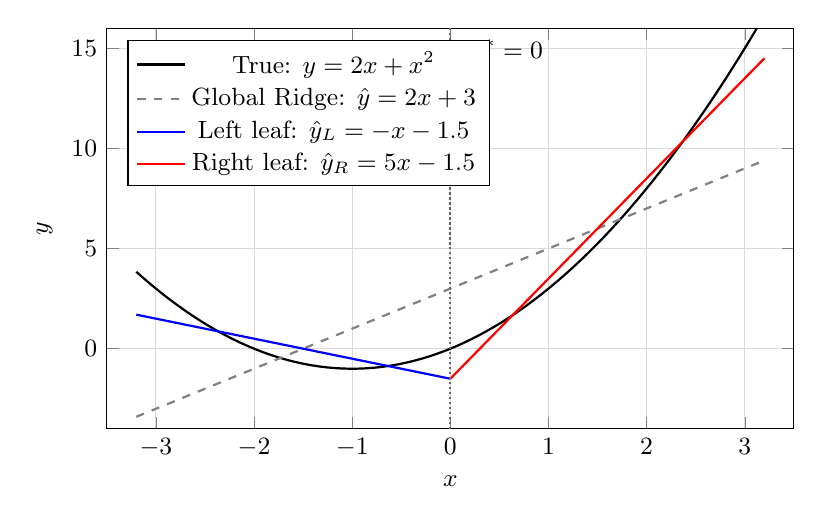
\begin{tikzpicture}
\begin{axis}[
    width=0.85\textwidth,
    height=0.55\textwidth,
    xlabel={$x$},
    ylabel={$y$},
    xmin=-3.5, xmax=3.5,
    ymin=-4, ymax=16,
    grid=major,
    grid style={gray!30},
    legend style={at={(0.03,0.97)}, anchor=north west, font=\small},
    tick label style={font=\small},
    label style={font=\small},
]

% True function: y = 2x + x^2
\addplot[
    domain=-3.2:3.2,
    samples=80,
    thick,
    black,
] {2*x + x^2};
\addlegendentry{True: $y = 2x + x^2$}

% Global Ridge fit: y = 2x + 3 (population-level: slope=2, intercept=E[x^2]=3)
\addplot[
    domain=-3.2:3.2,
    samples=2,
    dashed,
    thick,
    gray,
] {2*x + 3};
\addlegendentry{Global Ridge: $\hat{y} = 2x + 3$}

% Left leaf: y = -x - 1.5  (population Ridge on [-3,0])
\addplot[
    domain=-3.2:0,
    samples=2,
    thick,
    blue,
] {-1*x - 1.5};
\addlegendentry{Left leaf: $\hat{y}_L = -x - 1.5$}

% Right leaf: y = 5x - 1.5  (population Ridge on [0,3])
\addplot[
    domain=0:3.2,
    samples=2,
    thick,
    red,
] {5*x - 1.5};
\addlegendentry{Right leaf: $\hat{y}_R = 5x - 1.5$}

% Split point indicator
\draw[densely dotted, thick, black!60] (axis cs:0,-4) -- (axis cs:0,16);
\node[font=\small, anchor=south west] at (axis cs:0.1,14) {$\tau^* = 0$};

\end{axis}
\end{tikzpicture}
\caption{Analytical example with $d=1$ and $y = 2x + x^2$. The global Ridge fit (dashed grey) captures only the average linear trend. RHM with $\text{max\_depth}=1$ splits at $\tau^* = 0$ and fits population-level Ridge models on each half (blue, red), reducing the maximum pointwise error by $4\times$ relative to the global fit. All coefficients are closed-form population values.}\label{fig:example}
\end{figure}

This example illustrates the core mechanism: RHM identifies the axis of greatest variation (here the only feature), finds the split point that best separates distinct linear regimes, and fits local models that together approximate the non-linear surface far more accurately than any single linear model.

\subsection{Convergence with Increasing Depth}\label{sec:convergence}

The depth-1 example above shows a single split reducing MSE by 87\%. A natural question is: how does the approximation improve as we continue splitting? Figure~\ref{fig:depth_progression} answers this by showing the piecewise linear approximation of $y = 2x + x^2$ on $[-3,3]$ at depths 1 through 4, producing 2, 4, 8, and 16 leaf segments respectively.

On each segment $[a,b]$ of width $h = b - a$, the population-level Ridge fit has a closed-form solution: slope $\hat{\beta} = 2 + a + b$ (the average derivative of $2x + x^2$ on $[a,b]$) and intercept $\hat{\beta}_0 = -(a^2 + 4ab + b^2)/6$. A notable property of this idealised setting emerges: \emph{adjacent leaf models agree exactly at their shared boundary}. That is, for any two neighbouring segments $[a,m]$ and $[m,b]$ with $m = (a+b)/2$, the left and right Ridge fits predict the same value at $x = m$. The piecewise approximation is therefore continuous---a polygon that wraps smoothly around the parabola with no gaps at the split points. (On finite samples, small discontinuities will generally be present; see Section~\ref{sec:algorithm}, Structural Properties.)

\begin{figure}[ht]
\centering
\begin{minipage}[t]{0.48\textwidth}
\centering
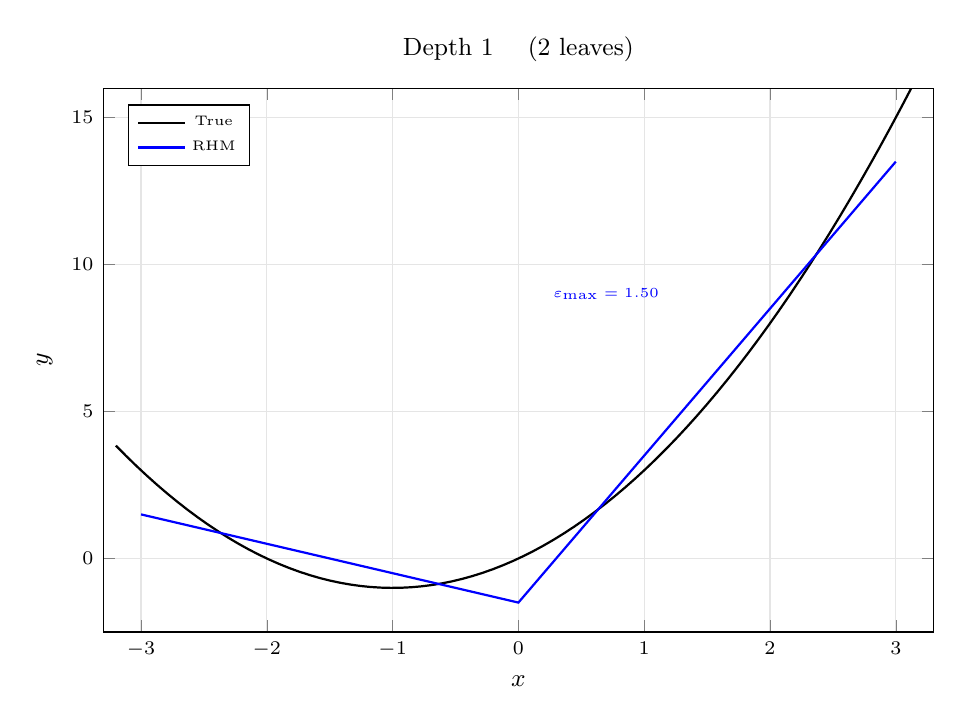
\begin{tikzpicture}
\begin{axis}[
    width=\textwidth, height=0.7\textwidth,
    xlabel={$x$}, ylabel={$y$},
    xmin=-3.3, xmax=3.3, ymin=-2.5, ymax=16,
    grid=major, grid style={gray!20},
    tick label style={font=\scriptsize},
    label style={font=\small},
    title={\small Depth 1 \quad (2 leaves)},
    title style={font=\small},
    legend style={at={(0.03,0.97)}, anchor=north west, font=\tiny},
]
\addplot[domain=-3.2:3.2, samples=80, thick, black] {2*x + x^2};
\addlegendentry{True}
\addplot[thick, blue] coordinates {
    (-3, 1.5) (0, -1.5) (3, 13.5)
};
\addlegendentry{RHM}
\node[font=\tiny, blue, anchor=west] at (axis cs:0.2,9) {$\varepsilon_{\max} = 1.50$};
\end{axis}
\end{tikzpicture}
\end{minipage}\hfill
\begin{minipage}[t]{0.48\textwidth}
\centering
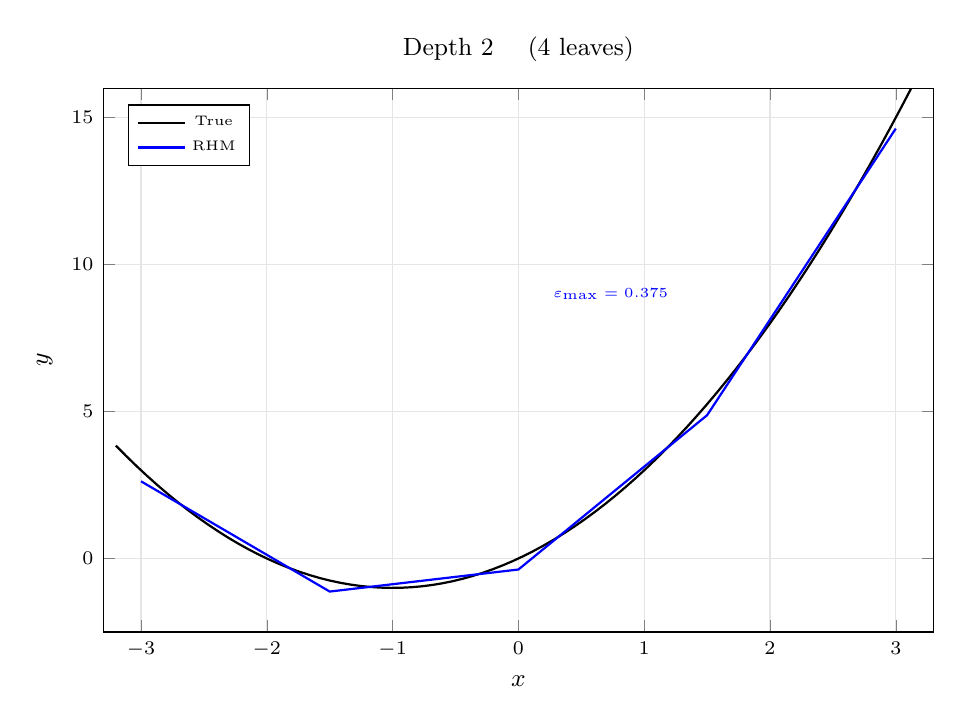
\begin{tikzpicture}
\begin{axis}[
    width=\textwidth, height=0.7\textwidth,
    xlabel={$x$}, ylabel={$y$},
    xmin=-3.3, xmax=3.3, ymin=-2.5, ymax=16,
    grid=major, grid style={gray!20},
    tick label style={font=\scriptsize},
    label style={font=\small},
    title={\small Depth 2 \quad (4 leaves)},
    title style={font=\small},
    legend style={at={(0.03,0.97)}, anchor=north west, font=\tiny},
]
\addplot[domain=-3.2:3.2, samples=80, thick, black] {2*x + x^2};
\addlegendentry{True}
\addplot[thick, blue] coordinates {
    (-3, 2.625) (-1.5, -1.125) (0, -0.375) (1.5, 4.875) (3, 14.625)
};
\addlegendentry{RHM}
\node[font=\tiny, blue, anchor=west] at (axis cs:0.2,9) {$\varepsilon_{\max} = 0.375$};
\end{axis}
\end{tikzpicture}
\end{minipage}

\vspace{6pt}

\begin{minipage}[t]{0.48\textwidth}
\centering
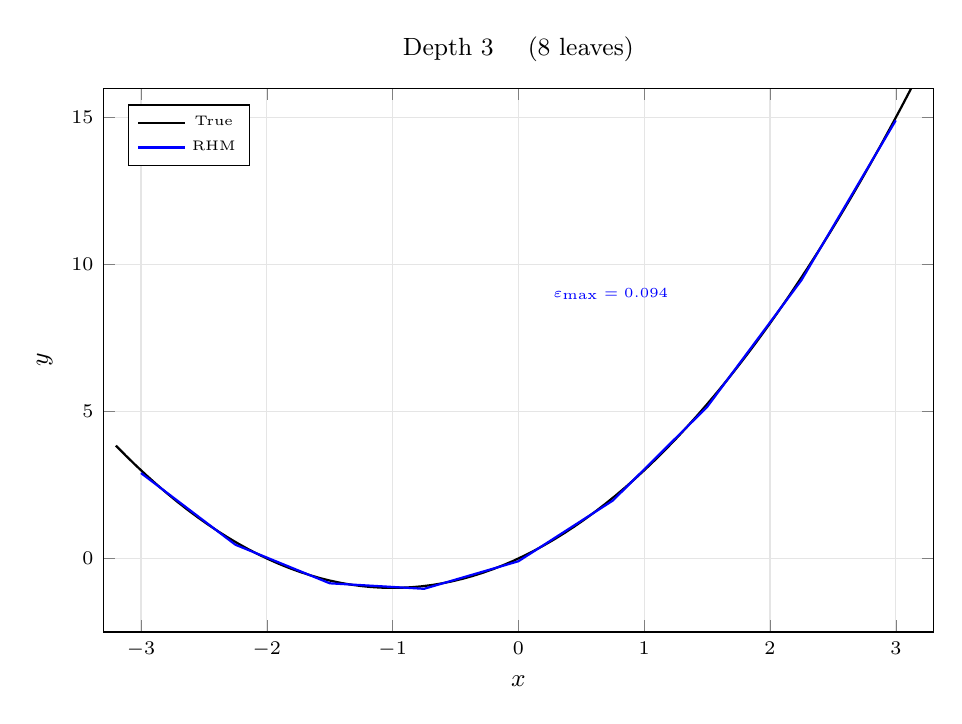
\begin{tikzpicture}
\begin{axis}[
    width=\textwidth, height=0.7\textwidth,
    xlabel={$x$}, ylabel={$y$},
    xmin=-3.3, xmax=3.3, ymin=-2.5, ymax=16,
    grid=major, grid style={gray!20},
    tick label style={font=\scriptsize},
    label style={font=\small},
    title={\small Depth 3 \quad (8 leaves)},
    title style={font=\small},
    legend style={at={(0.03,0.97)}, anchor=north west, font=\tiny},
]
\addplot[domain=-3.2:3.2, samples=80, thick, black] {2*x + x^2};
\addlegendentry{True}
\addplot[thick, blue] coordinates {
    (-3, 2.906) (-2.25, 0.469) (-1.5, -0.844)
    (-0.75, -1.031) (0, -0.094) (0.75, 1.969)
    (1.5, 5.156) (2.25, 9.469) (3, 14.906)
};
\addlegendentry{RHM}
\node[font=\tiny, blue, anchor=west] at (axis cs:0.2,9) {$\varepsilon_{\max} = 0.094$};
\end{axis}
\end{tikzpicture}
\end{minipage}\hfill
\begin{minipage}[t]{0.48\textwidth}
\centering
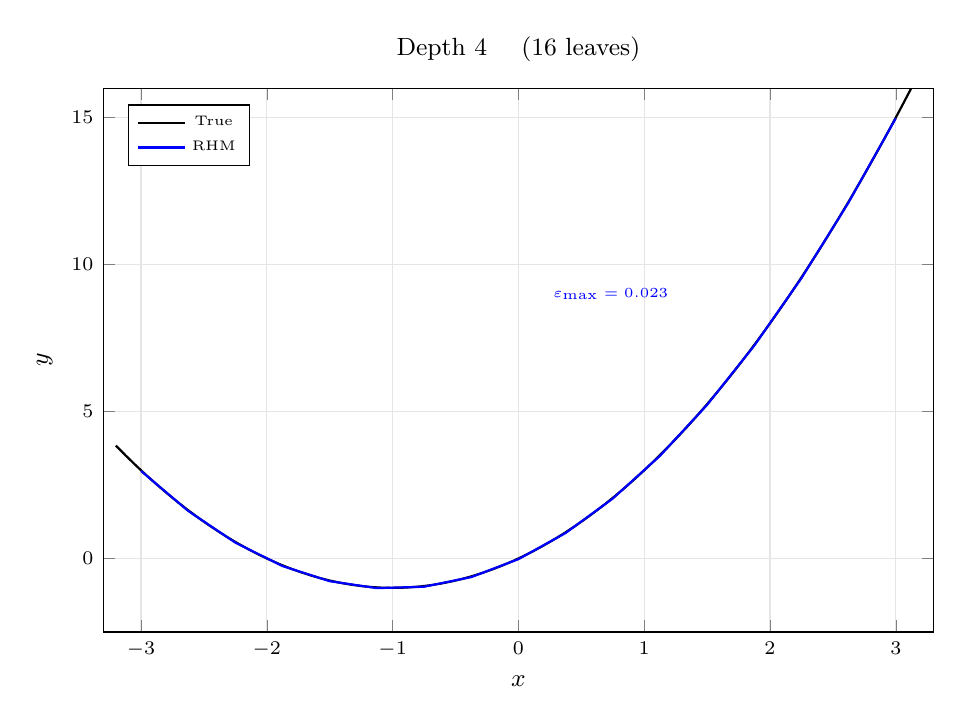
\begin{tikzpicture}
\begin{axis}[
    width=\textwidth, height=0.7\textwidth,
    xlabel={$x$}, ylabel={$y$},
    xmin=-3.3, xmax=3.3, ymin=-2.5, ymax=16,
    grid=major, grid style={gray!20},
    tick label style={font=\scriptsize},
    label style={font=\small},
    title={\small Depth 4 \quad (16 leaves)},
    title style={font=\small},
    legend style={at={(0.03,0.97)}, anchor=north west, font=\tiny},
]
\addplot[domain=-3.2:3.2, samples=80, thick, black] {2*x + x^2};
\addlegendentry{True}
\addplot[thick, blue] coordinates {
    (-3, 2.977) (-2.625, 1.617) (-2.25, 0.539)
    (-1.875, -0.258) (-1.5, -0.773) (-1.125, -1.008)
    (-0.75, -0.961) (-0.375, -0.633) (0, -0.023)
    (0.375, 0.867) (0.75, 2.039) (1.125, 3.492)
    (1.5, 5.227) (1.875, 7.242) (2.25, 9.539)
    (2.625, 12.117) (3, 14.977)
};
\addlegendentry{RHM}
\node[font=\tiny, blue, anchor=west] at (axis cs:0.2,9) {$\varepsilon_{\max} = 0.023$};
\end{axis}
\end{tikzpicture}
\end{minipage}
\caption{Piecewise linear approximation of $y = 2x + x^2$ at increasing tree depth. At each depth $k$, the interval $[-3,3]$ is partitioned into $2^k$ segments. The approximation (blue polyline) wraps progressively tighter around the true parabola (black curve), with no discontinuities at segment boundaries. The maximum error $\varepsilon_{\max}$ decreases by a factor of 4 with each depth level.}\label{fig:depth_progression}
\end{figure}

The maximum approximation error on each segment is $h^2/6$, where $h$ is the segment width. Since each depth level halves $h$, the error decreases by a factor of four per level (Table~\ref{tab:convergence}). This is the classical $O(h^2)$ convergence rate of piecewise linear approximation applied to smooth ($C^2$) functions.

\begin{table}[ht]
\centering
\caption{Convergence of the piecewise linear approximation with tree depth.}\label{tab:convergence}
\begin{tabular}{ccccc}
\toprule
\textbf{Depth} & \textbf{Leaves} & \textbf{Segment width $h$} & \textbf{Max error $h^2/6$} & \textbf{Reduction} \\
\midrule
1 & 2  & 3.000 & 1.500 & --- \\
2 & 4  & 1.500 & 0.375 & $4\times$ \\
3 & 8  & 0.750 & 0.094 & $4\times$ \\
4 & 16 & 0.375 & 0.023 & $4\times$ \\
\bottomrule
\end{tabular}
\end{table}

The continuity at boundaries is a consequence of the symmetry of the quadratic: when a segment is split at its midpoint, the two child Ridge fits yield identical predictions at the split point. This property holds exactly for quadratic targets and approximately for smooth functions with moderate higher-order derivatives.

\subsection{Extension to Two Dimensions}

For the separable function $y = 3x_1 - 2x_2 + x_1^2 + x_2^2$, the same convergence applies independently along each axis. Figure~\ref{fig:partition_2d} shows the partition of $[-2,2]^2$ produced by RHM at depth~2. The algorithm adapts its splitting axis at each node based on the Ridge coefficients: the root splits on $x_1$ (since $|\hat{\beta}_1| = 3 > |\hat{\beta}_2| = 2$); the left child, where the quadratic $x_1^2$ has reduced $|\hat{\beta}_1|$ to~1, switches to splitting on $x_2$ ($|\hat{\beta}_2| = 2$ now dominates); the right child, where $x_1^2$ has amplified $|\hat{\beta}_1|$ to~5, continues splitting on $x_1$.

\begin{figure}[ht]
\centering
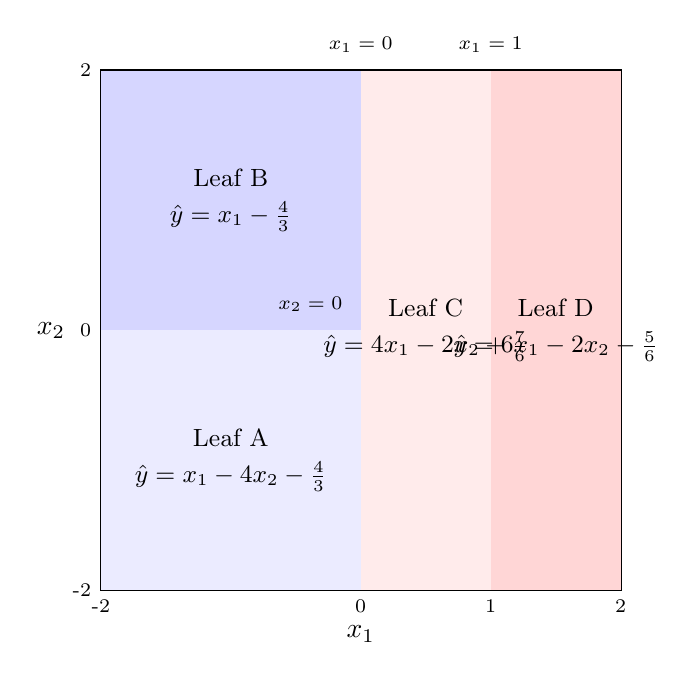
\begin{tikzpicture}[scale=1.1]
% Outer rectangle
\draw[thick] (-3,-3) rectangle (3,3);

% Axis labels
\node[below] at (0,-3.3) {$x_1$};
\node[left] at (-3.3,0) {$x_2$};

% Tick marks and labels
\foreach \v/\l in {-3/-2, 0/0, 3/2} {
    \node[below, font=\scriptsize] at (\v,-3) {\l};
    \node[left, font=\scriptsize] at (-3,\v) {\l};
}
\node[below, font=\scriptsize] at (1.5,-3) {1};

% Split lines
\draw[thick, dashed] (0,-3) -- (0,3);        % root split: x1 = 0
\draw[thick, dashed] (-3,0) -- (0,0);         % left child split: x2 = 0
\draw[thick, dashed] (1.5,-3) -- (1.5,3);     % right child split: x1 = 1

% Region shading
\fill[blue!8] (-3,-3) rectangle (0,0);
\fill[blue!16] (-3,0) rectangle (0,3);
\fill[red!8] (0,-3) rectangle (1.5,3);
\fill[red!16] (1.5,-3) rectangle (3,3);

% Region labels
\node[font=\small, align=center] at (-1.5,-1.5) {Leaf A\\[2pt]$\hat{y} = x_1 - 4x_2 - \tfrac{4}{3}$};
\node[font=\small, align=center] at (-1.5,1.5) {Leaf B\\[2pt]$\hat{y} = x_1 - \tfrac{4}{3}$};
\node[font=\small, align=center] at (0.75,0) {Leaf C\\[2pt]$\hat{y} = 4x_1 - 2x_2 + \tfrac{7}{6}$};
\node[font=\small, align=center] at (2.25,0) {Leaf D\\[2pt]$\hat{y} = 6x_1 - 2x_2 - \tfrac{5}{6}$};

% Split annotations
\node[font=\scriptsize, anchor=south] at (0,3.1) {$x_1 = 0$};
\node[font=\scriptsize, anchor=south east] at (-0.1,0.1) {$x_2 = 0$};
\node[font=\scriptsize, anchor=south] at (1.5,3.1) {$x_1 = 1$};

\end{tikzpicture}
\caption{Partition of $[-2,2]^2$ by RHM at depth~2 for $y = 3x_1 - 2x_2 + x_1^2 + x_2^2$. The root splits on $x_1$ at~0. The left child splits on $x_2$ at~0 (where $x_2$ dominates after the $x_1^2$ curvature reduces $|\hat{\beta}_1|$). The right child splits on $x_1$ at~1 (where $x_1$ still dominates). Each leaf shows its fitted Ridge plane. The adaptive axis selection at each node is a distinguishing feature of the coefficient-guided heuristic.}\label{fig:partition_2d}
\end{figure}

With increasing depth, the tree continues to subdivide each region along the axis with the largest Ridge coefficient, producing smaller rectangular cells whose Ridge planes approximate the paraboloid with $O(h^2)$ error in each axis.

\paragraph{Surface approximation with 32 leaf planes.}
Figure~\ref{fig:surface_comparison} demonstrates this convergence in two dimensions. We partition $[-2,2]^2$ into an $8 \times 4$ grid of 32 rectangular cells---equivalent to a depth-5 tree with alternating axis splits (5 levels produce $2^5 = 32$ leaves, distributed as 8 strips in $x_1$ and 4 strips in $x_2$). On each cell $[a_1, b_1] \times [a_2, b_2]$, the Ridge fit has closed-form coefficients:
\[
    \hat{\beta}_1 = 3 + a_1 + b_1, \quad \hat{\beta}_2 = -2 + a_2 + b_2, \quad \hat{\beta}_0 = -\tfrac{a_1^2 + 4a_1 b_1 + b_1^2}{6} - \tfrac{a_2^2 + 4a_2 b_2 + b_2^2}{6}.
\]
Because the target is separable, adjacent cells produce Ridge planes that \emph{agree exactly at their shared boundary}---the 32-plane surface is fully continuous. The maximum error is $h_1^2/6 + h_2^2/6 \approx 0.042 + 0.167 = 0.21$ (with $h_1 = 0.5$ in $x_1$, $h_2 = 1.0$ in $x_2$).

\begin{figure}[ht]
\centering
\begin{minipage}[t]{0.48\textwidth}
\centering
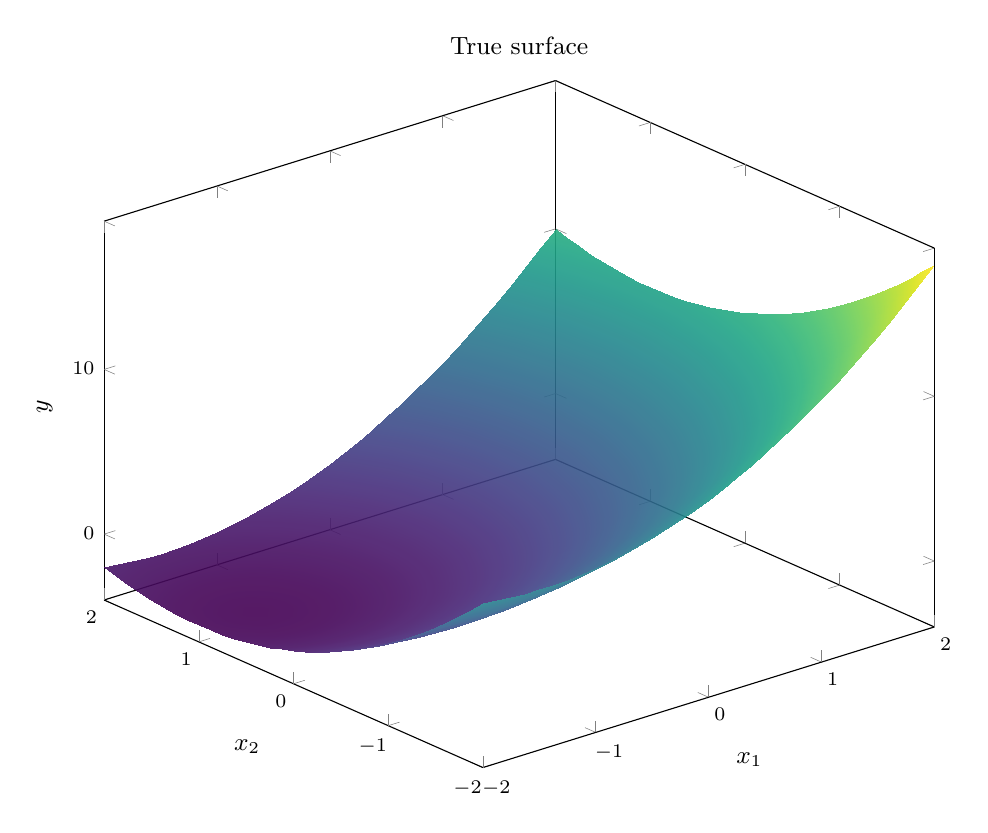
\begin{tikzpicture}
\begin{axis}[
    width=\textwidth, height=0.85\textwidth,
    view={-40}{30},
    xlabel={$x_1$}, ylabel={$x_2$}, zlabel={$y$},
    title={\small True surface},
    title style={at={(0.5,1.0)}, font=\small},
    colormap/viridis,
    tick label style={font=\scriptsize},
    label style={font=\small},
    zmin=-4, zmax=19,
]
\addplot3[
    surf, shader=interp,
    domain=-2:2, domain y=-2:2,
    samples=33, opacity=0.9,
] {3*x - 2*y + x^2 + y^2};
\end{axis}
\end{tikzpicture}
\end{minipage}\hfill
\begin{minipage}[t]{0.48\textwidth}
\centering
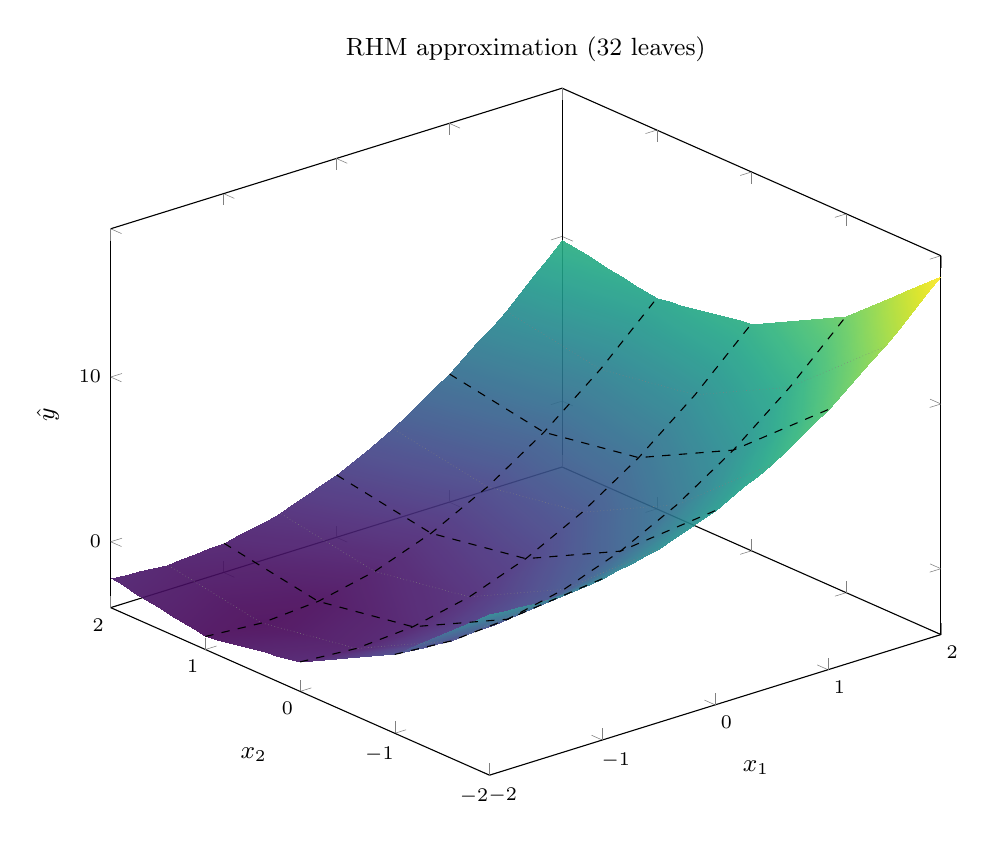
\begin{tikzpicture}
\begin{axis}[
    width=\textwidth, height=0.85\textwidth,
    view={-40}{30},
    xlabel={$x_1$}, ylabel={$x_2$}, zlabel={$\hat{y}$},
    title={\small RHM approximation (32 leaves)},
    title style={at={(0.5,1.0)}, font=\small},
    colormap/viridis,
    tick label style={font=\scriptsize},
    label style={font=\small},
    zmin=-4, zmax=19,
]
\addplot3[
    surf, shader=interp,
    domain=-2:2, domain y=-2:2,
    samples=33, opacity=0.9,
] {%
    ((x<-1.5)*(-0.5*x - 3.0417)
    + (x>=-1.5)*(x<-1)*(0.5*x - 1.5417)
    + (x>=-1)*(x<-0.5)*(1.5*x - 0.5417)
    + (x>=-0.5)*(x<0)*(2.5*x - 0.0417)
    + (x>=0)*(x<0.5)*(3.5*x - 0.0417)
    + (x>=0.5)*(x<1)*(4.5*x - 0.5417)
    + (x>=1)*(x<1.5)*(5.5*x - 1.5417)
    + (x>=1.5)*(6.5*x - 3.0417))
    +
    ((y<-1)*(-5*y - 2.1667)
    + (y>=-1)*(y<0)*(-3*y - 0.1667)
    + (y>=0)*(y<1)*(-1*y - 0.1667)
    + (y>=1)*(1*y - 2.1667))
};
% Grid lines on the surface at x1 = -1, 0, 1 (major)
\addplot3[black, thin, dashed] coordinates {
    (-1,-2,5.79) (-1,-1,0.79) (-1,0,-2.21) (-1,1,-3.21) (-1,2,-2.21)};
\addplot3[black, thin, dashed] coordinates {
    (0,-2,7.79) (0,-1,2.79) (0,0,-0.21) (0,1,-1.21) (0,2,-0.21)};
\addplot3[black, thin, dashed] coordinates {
    (1,-2,11.79) (1,-1,6.79) (1,0,3.79) (1,1,2.79) (1,2,3.79)};
% Grid lines at x1 = -1.5, -0.5, 0.5, 1.5 (fine)
\addplot3[black!50, very thin, densely dotted] coordinates {
    (-1.5,-2,5.54) (-1.5,-1,0.54) (-1.5,0,-2.46) (-1.5,1,-3.46) (-1.5,2,-2.46)};
\addplot3[black!50, very thin, densely dotted] coordinates {
    (-0.5,-2,6.54) (-0.5,-1,1.54) (-0.5,0,-1.46) (-0.5,1,-2.46) (-0.5,2,-1.46)};
\addplot3[black!50, very thin, densely dotted] coordinates {
    (0.5,-2,9.54) (0.5,-1,4.54) (0.5,0,1.54) (0.5,1,0.54) (0.5,2,1.54)};
\addplot3[black!50, very thin, densely dotted] coordinates {
    (1.5,-2,14.54) (1.5,-1,9.54) (1.5,0,6.54) (1.5,1,5.54) (1.5,2,6.54)};
% Grid lines at x2 = -1, 0, 1
\addplot3[black, thin, dashed] coordinates {
    (-2,-1,0.79) (-1.5,-1,0.54) (-1,-1,0.79) (-0.5,-1,1.54)
    (0,-1,2.79) (0.5,-1,4.54) (1,-1,6.79) (1.5,-1,9.54) (2,-1,12.79)};
\addplot3[black, thin, dashed] coordinates {
    (-2,0,-2.21) (-1.5,0,-2.46) (-1,0,-2.21) (-0.5,0,-1.46)
    (0,0,-0.21) (0.5,0,1.54) (1,0,3.79) (1.5,0,6.54) (2,0,9.79)};
\addplot3[black, thin, dashed] coordinates {
    (-2,1,-3.21) (-1.5,1,-3.46) (-1,1,-3.21) (-0.5,1,-2.46)
    (0,1,-1.21) (0.5,1,0.54) (1,1,2.79) (1.5,1,5.54) (2,1,8.79)};
\end{axis}
\end{tikzpicture}
\end{minipage}
\caption{True surface $y = 3x_1 - 2x_2 + x_1^2 + x_2^2$ (left) and RHM piecewise planar approximation with 32 leaves on an $8\!\times\!4$ grid (right). Dashed lines mark the $4\!\times\!4$ major cell boundaries; dotted lines mark the finer $x_1$ subdivisions. The 32 Ridge planes are continuous across all boundaries and closely wrap the paraboloid with maximum error $\approx 0.21$.}\label{fig:surface_comparison}
\end{figure}

\paragraph{Error convergence with depth.}
Figure~\ref{fig:error_convergence} quantifies the approximation error as a function of tree depth for both the one-dimensional ($d\!=\!1$) and two-dimensional ($d\!=\!2$) examples. In one dimension, each depth level halves the segment width $h$, reducing the maximum error $h^2/6$ by a factor of four---yielding a straight line of slope $-2$ on the log-log plot. In two dimensions with alternating axis splits, the error decreases by a factor of four every \emph{two} depth levels (since only one axis is refined per level), producing a shallower slope of $-1$ on the log-log scale. At depth 8, the one-dimensional error ($9.2 \times 10^{-5}$) and two-dimensional error ($0.021$) are both negligible relative to the function's range.

\begin{figure}[ht]
\centering
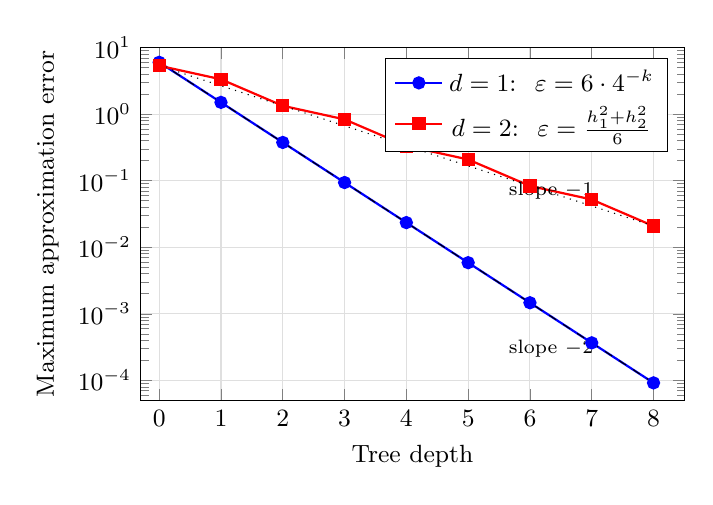
\begin{tikzpicture}
\begin{axis}[
    width=0.7\textwidth, height=0.5\textwidth,
    xlabel={Tree depth},
    ylabel={Maximum approximation error},
    ymode=log,
    xmin=-0.3, xmax=8.5,
    ymin=0.00005, ymax=10,
    grid=major, grid style={gray!25},
    tick label style={font=\small},
    label style={font=\small},
    legend style={at={(0.97,0.97)}, anchor=north east, font=\small},
    xtick={0,1,2,3,4,5,6,7,8},
]
% 1D: error = 6 / 4^depth
\addplot[thick, blue, mark=*, mark size=2pt] coordinates {
    (0, 6.0) (1, 1.5) (2, 0.375) (3, 0.09375)
    (4, 0.02344) (5, 0.005859) (6, 0.001465)
    (7, 0.000366) (8, 0.0000916)
};
\addlegendentry{$d=1$: $\;\varepsilon = 6 \cdot 4^{-k}$}

% 2D: alternating axis splits
\addplot[thick, red, mark=square*, mark size=2pt] coordinates {
    (0, 5.333) (1, 3.333) (2, 1.333) (3, 0.833)
    (4, 0.333) (5, 0.208) (6, 0.0833)
    (7, 0.0521) (8, 0.0208)
};
\addlegendentry{$d=2$: $\;\varepsilon = \tfrac{h_1^2 + h_2^2}{6}$}

% Reference slope lines
\addplot[black, dashed, thin, domain=0:8, samples=2] {6*2^(-2*x)};
\addplot[black, dotted, thin, domain=0:8, samples=2] {5.333*2^(-x)};

\node[font=\scriptsize, anchor=west] at (axis cs:5.5, 0.0003) {slope $-2$};
\node[font=\scriptsize, anchor=west] at (axis cs:5.5, 0.07) {slope $-1$};

\end{axis}
\end{tikzpicture}
\caption{Maximum approximation error versus tree depth for $d=1$ (blue circles) and $d=2$ (red squares) on a semi-log scale. In one dimension, each depth level reduces the error by $4\times$ (slope $-2$ on a log-log scale, shown dashed). In two dimensions with alternating axis splits, the error halves per depth level on average (slope $-1$, shown dotted), because each level refines only one axis. Both curves confirm the theoretical $O(h^2)$ convergence rate.}\label{fig:error_convergence}
\end{figure}

\section{Complexity Analysis}\label{sec:complexity}

\subsection{Training Time}

Let $n$ = training samples, $d$ = features, $T$ = number of nodes, $D$ = \texttt{max\_depth}. At each internal node with $n_v$ samples:
\begin{itemize}
    \item \textbf{Feature selection:} One Ridge fit costs $O(n_v d^2)$. Argmax over $d$ coefficients costs $O(d)$. Total: $O(n_v d^2)$.
    \item \textbf{Split-point search:} 9 candidate splits, each requiring two Ridge fits. Cost: $O(9 \times 2 \times n_v d^2) = O(n_v d^2)$.
\end{itemize}
Because the left and right partitions together contain $n_v$ samples and each sample appears in exactly one partition per level, the total work per depth level is $O(nd^2)$. Across $D$ levels the total training cost is:
\[
    O(D \cdot n \cdot d^2)
\]
This is linear in depth and quadratic in features, making RHM tractable for moderate $d$ and small-to-medium $D$.

\subsection{Inference Time}

Each test sample traverses a path of at most $D + 1$ nodes and then executes one Ridge prediction of $O(d)$. Per-sample inference cost is $O(D + d)$. For $m$ test samples: $O(m(D + d))$.

\subsection{Space Complexity}

The tree contains at most $2^{D+1} - 1$ nodes. Each leaf stores a Ridge model with $O(d)$ parameters. Internal nodes store only a feature index and scalar threshold. Total space: $O(2^D \cdot d)$.

\section{From RHM to ACGMT}\label{sec:acgmt}

\subsection{Limitations of Top-1 Feature Selection}

The preceding analysis shows that RHM converges correctly in idealised, low-dimensional settings where the splitting axis is unambiguous. In more realistic regression problems, however, the top-1 feature selection heuristic is brittle in several important ways.

\paragraph{Sensitivity to feature scaling.} Ridge coefficients are scale-dependent: a feature measured in large units will receive a proportionally small coefficient even if it is the most predictive axis. Without pre-standardization, the coefficient ranking can be dominated by the scale of the features rather than their predictive relevance.

\paragraph{Fragility under collinearity.} When two predictive features are highly correlated, Ridge regression distributes their joint signal across both coefficients, each reduced in magnitude. The top-1 selection may commit to the feature that happened to receive a slightly larger share of this divided signal, discarding a potentially equally or more useful splitting axis.

\paragraph{Regime-dependent structure.} In problems where the response is piecewise linear with distinct breakpoints that are not aligned with the single largest-coefficient feature, the top-1 heuristic will systematically fail to identify useful splits, producing large residual errors in the affected partitions.

These failure modes motivate a more flexible search strategy that uses coefficient magnitudes as a \emph{screening tool} rather than a hard, irrevocable commitment. This is precisely the design goal of ACGMT.

\subsection{Algorithm}

Let $(X, y)$ denote the data at a node, with $X \in \mathbb{R}^{n \times d}$ and $y \in \mathbb{R}^n$. ACGMT preserves the overall RHM structure but changes the split search from a single-axis decision to a screened multi-axis evaluation. Figure~\ref{fig:concept} illustrates the structural difference.

\begin{figure}[ht]
\centering
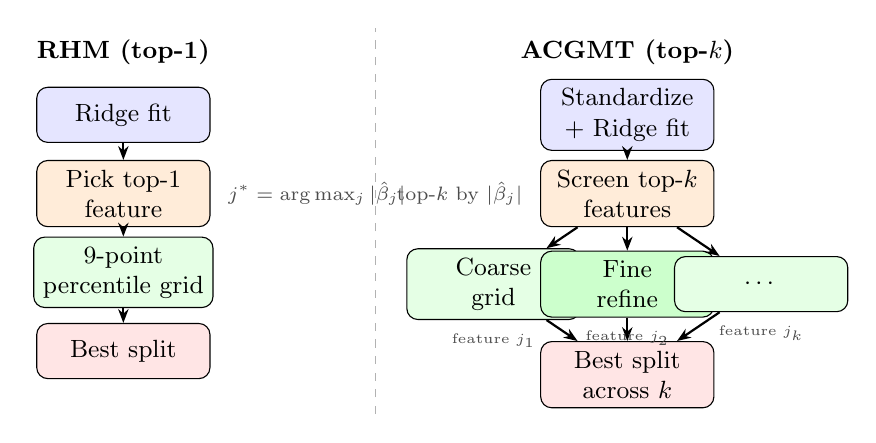
\begin{tikzpicture}[
    box/.style={draw, rounded corners, minimum width=2.2cm, minimum height=0.7cm, font=\small, align=center},
    arrow/.style={-{Stealth[length=5pt]}, thick},
    label/.style={font=\scriptsize, text=black!70},
]
% RHM side
\node[font=\small\bfseries] at (-3.2, 3.8) {RHM (top-1)};
\node[box, fill=blue!10] (r1) at (-3.2, 3) {Ridge fit};
\node[box, fill=orange!15] (r2) at (-3.2, 2) {Pick top-1\\feature};
\node[box, fill=green!10] (r3) at (-3.2, 1) {9-point\\percentile grid};
\node[box, fill=red!10] (r4) at (-3.2, 0) {Best split};

\draw[arrow] (r1) -- (r2);
\draw[arrow] (r2) -- (r3);
\draw[arrow] (r3) -- (r4);
\node[label, right=0.1cm of r2] {$j^* = \arg\max_j |\hat\beta_j|$};

% ACGMT side
\node[font=\small\bfseries] at (3.2, 3.8) {ACGMT (top-$k$)};
\node[box, fill=blue!10] (a1) at (3.2, 3) {Standardize\\+ Ridge fit};
\node[box, fill=orange!15] (a2) at (3.2, 2) {Screen top-$k$\\features};
\node[box, fill=green!10] (a3a) at (1.5, 0.85) {Coarse\\grid};
\node[box, fill=green!20] (a3b) at (3.2, 0.85) {Fine\\refine};
\node[box, fill=green!10] (a3c) at (4.9, 0.85) {$\cdots$};
\node[box, fill=red!10] (a4) at (3.2, -0.3) {Best split\\across $k$};

\draw[arrow] (a1) -- (a2);
\draw[arrow] (a2) -- (a3a);
\draw[arrow] (a2) -- (a3b);
\draw[arrow] (a2) -- (a3c);
\draw[arrow] (a3a) -- (a4);
\draw[arrow] (a3b) -- (a4);
\draw[arrow] (a3c) -- (a4);
\node[label, left=0.1cm of a2] {top-$k$ by $|\hat\beta_j|$};
\node[label, below=0.05cm of a3a, font=\tiny] {feature $j_1$};
\node[label, below=0.05cm of a3b, font=\tiny] {feature $j_2$};
\node[label, below=0.05cm of a3c, font=\tiny] {feature $j_k$};

% Divider
\draw[dashed, black!30] (0, -0.8) -- (0, 4.1);
\end{tikzpicture}
\caption{Conceptual comparison of split selection at a single node. RHM (left) commits to one feature and searches a fixed grid. ACGMT (right) standardizes features, screens the top-$k$ by coefficient magnitude, searches each with optional coarse-to-fine refinement, and selects the best split across all $k$ candidates.}\label{fig:concept}
\end{figure}

\paragraph{Step 1: coefficient-guided feature screening.}
If standardization is enabled, ACGMT centers and scales the node features column-wise before fitting Ridge. Let $\hat{\beta}$ denote the fitted coefficient vector. The algorithm ranks features by $|\hat{\beta}_j|$ and keeps the top-$k$ candidates rather than only the single largest one.

\paragraph{Step 2: threshold search within screened features.}
For each retained feature, ACGMT first evaluates a coarse quantile grid. In our implementation, the coarse grid matches the 10th through 90th percentiles used by RHM. If adaptive refinement is enabled, the best coarse threshold is then refined by searching a smaller local window with a denser secondary grid.

\paragraph{Step 3: split selection.}
For every candidate threshold $\tau$, the node is partitioned into left and right subsets and two child Ridge models are fit. The score is the weighted in-sample child MSE,
\[
\mathrm{MSE}(\tau) =
\frac{|L| \cdot \mathrm{MSE}_L + |R| \cdot \mathrm{MSE}_R}{n}.
\]
The feature-threshold pair with minimum score is selected, subject to the minimum node size constraint.

\paragraph{Step 4: recursion and pruning.}
Tree growth proceeds recursively until the depth limit or minimum sample constraint is reached. If pruning is enabled, the tree is first grown on a build split and then pruned bottom-up using a held-out validation subset. A subtree is collapsed into a single Ridge leaf whenever the leaf's validation MSE is no worse than the subtree's validation MSE on the validation samples that reach that node.

\subsection{Variants Studied}

The experiments study four ACGMT variants:
\begin{itemize}
    \item \textbf{ACGMT (top1, no-std):} top-$1$ feature selection, no standardization, fixed grid, no pruning. This is the closest ACGMT analogue to RHM.
    \item \textbf{ACGMT (top3, std):} top-$3$ features, standardization, fixed grid, no pruning.
    \item \textbf{ACGMT (full):} top-$3$ features with standardization,
    adaptive threshold refinement, and validation-aware pruning.
    \item \textbf{Ablation variants:} versions that isolate top-$k$, standardization, adaptive grid search, and pruning separately.
\end{itemize}

\subsection{Complexity}

For fixed $k$, fixed coarse grid size, and fixed fine grid size, ACGMT has the same asymptotic training order as RHM up to a larger constant factor. Each internal node now fits one Ridge model for ranking and then evaluates up to $k$ features across a bounded set of candidate thresholds. Thus, compared with RHM, ACGMT spends more computation per node but remains far cheaper than exhaustive search over all features and thresholds. For the settings used here, the practical fit-time overhead is modest relative to gradient boosting, while still preserving the single-tree structure.

\section{Experimental Evaluation}\label{sec:experiments}

\subsection{RHM Baseline Evaluation}

\subsubsection{Synthetic Data Generation}

To evaluate RHM in a controlled setting, we generate synthetic data with known linear, quadratic, and interaction structure. The target variable is:
\[
    y = 5x_1 - 3x_2 + \sum_{i=3}^{10} x_i + 0.5x_1^2 + 0.3x_2^2 + 2x_3 x_4 + \varepsilon, \quad \varepsilon \sim \mathcal{N}(0, 0.5)
\]
where $x_i \sim \mathcal{N}(0, 1)$ i.i.d., $n = 5{,}000$ samples, $d = 10$ features. The quadratic and interaction terms are non-linear and cannot be captured by a global linear model, making this a suitable benchmark for assessing the benefit of local partitioning. Data are split 80/20 into training and test sets. All experiments use a fixed random seed (42) for reproducibility.

The baseline is a global Ridge regression ($\alpha = 1.0$) fitted on the full training set, and RHM is evaluated at $\text{max\_depth} \in \{1, 2, 3, 4\}$ with $\text{min\_samples\_split} = 100$ throughout.

\subsubsection{Results}

Table~\ref{tab:results} summarises the performance of the global Ridge baseline and RHM across depth levels.

\begin{table}[ht]
\centering
\caption{Test and training performance of RHM vs.\ Ridge baseline.}\label{tab:results}
\begin{tabular}{lcccc}
\toprule
\textbf{Model / Depth} & \textbf{Train MSE} & \textbf{Test MSE} & \textbf{Train $R^2$} & \textbf{Test $R^2$} \\
\midrule
Ridge (baseline) & 4.9196 & 5.2845 & 0.8951 & 0.8849 \\
RHM, depth=1     & 4.4381 & 4.8798 & 0.9053 & 0.8938 \\
RHM, depth=2     & 4.2716 & 4.8746 & 0.9089 & 0.8939 \\
RHM, depth=3     & 4.1593 & 4.9433 & 0.9113 & 0.8924 \\
RHM, depth=4     & 4.0127 & 5.0727 & 0.9144 & 0.8896 \\
\bottomrule
\end{tabular}
\end{table}

Deeper trees capture the quadratic and interaction structure more accurately on training data, with train MSE decreasing monotonically from 4.92 (Ridge) to 4.01 (depth=4). On test data, RHM achieves its best performance at depth=2 (test MSE 4.87, $R^2$ 0.894), after which test MSE increases slightly---consistent with mild overfitting as tree depth grows and leaf partitions shrink.

For $\text{max\_depth} = 2$, four leaf models are fitted. Because $x_1$ has the largest Ridge coefficient at both the root and both depth-1 children (its linear coefficient of 5 dominates the other features), the tree splits on $x_1$ at all internal nodes---first near $x_1 \approx 0.0$, then near $x_1 \approx -0.8$ (left child) and $x_1 \approx 1.3$ (right child). This produces four vertical strips along the $x_1$ axis rather than a grid across two features. Exporting the leaf coefficients reveals how the $x_1$ coefficient adapts across strips: it is smallest in the far-left partition (where $x_1 < -0.8$ and the quadratic $0.5\,x_1^2$ flattens the effective slope) and largest in the far-right partition (where $x_1 > 1.3$ and the quadratic steepens it). Coefficients on other features remain relatively stable across leaves, since the data-generating process couples non-linearity primarily to $x_1$ and $x_2$.

\subsection{ACGMT Stress Tests}

\subsubsection{Datasets}

We evaluate on five synthetic regression problems designed to stress specific failure modes of coefficient-guided splitting:
\begin{itemize}
    \item \textbf{Scaling:} features live on widely different numeric scales;
    \item \textbf{Correlated:} predictive features are paired with highly correlated surrogates;
    \item \textbf{Irrelevant:} a small number of relevant features are embedded among many irrelevant ones;
    \item \textbf{Interaction:} the response includes regime-dependent interaction effects;
    \item \textbf{Regime:} the response is piecewise linear with multiple breakpoints.
\end{itemize}
Each dataset contains 5{,}000 samples and is split 80/20 into train and test. We run 5 random seeds for every dataset-model pair and report means across seeds.

\subsubsection{Baselines}

We compare against:
\begin{itemize}
    \item Ridge regression;
    \item CART regression trees;
    \item Random Forest;
    \item Gradient Boosting regression trees;
    \item the original RHM implementation from Section~\ref{sec:algorithm}.
\end{itemize}
Random Forest uses single-threaded fitting in order to make fit-time comparisons less misleading. We emphasize fit time rather than prediction time when discussing efficiency, because the current RHM implementation uses slower row-wise prediction while ACGMT uses vectorized prediction.

\subsubsection{Protocol Details}

All non-pruned ACGMT variants train on the full training set. The pruned \texttt{ACGMT (full)} variant uses an 80/20 build/validation split within the training data, so its tree is grown on 80\% of the nominal training set and pruned using the held-out 20\%. The pruning ablation compares pruned and unpruned models built on the same 80\% subset, so only the pruning step differs.

\subsubsection{Main Comparison}

Table~\ref{tab:main} reports test MSE and fit time. The headline result is that adaptive coefficient-guided search substantially improves over RHM on datasets where top-1 feature commitment fails, especially the interaction and regime settings. RHM attains test MSE 4.746 on the interaction dataset and 2.791 on the regime dataset, while \texttt{ACGMT (top3, std)} reduces these to 0.385 and 0.352 respectively. The full pruned variant further improves the correlated and regime datasets, reaching 0.253 and 0.325.

\begin{table}[ht]
\centering
\caption{Main comparison across datasets. Test MSE is lower-is-better. Fit time is mean wall-clock training time in seconds.}\label{tab:main}
\resizebox{\textwidth}{!}{
\begin{tabular}{lcccccccc}
\toprule
\textbf{Dataset} & \textbf{Ridge} & \textbf{CART} & \textbf{RF} & \textbf{GBT} & \textbf{RHM} & \textbf{ACGMT top1} & \textbf{ACGMT top3+std} & \textbf{ACGMT full} \\
\midrule
\multicolumn{9}{c}{\textit{Test MSE}}\\
\midrule
correlated  & 0.711 & 2.784 & 2.068 & 0.335 & 0.277 & 0.277 & 0.259 & 0.253 \\
interaction & 5.102 & 1.947 & 1.387 & 0.352 & 4.746 & 4.746 & 0.385 & 0.389 \\
irrelevant  & 1.810 & 7.424 & 5.002 & 0.453 & 0.316 & 0.316 & 0.303 & 0.310 \\
regime      & 2.758 & 0.950 & 0.820 & 0.274 & 2.791 & 2.791 & 0.352 & 0.325 \\
scaling     & 6.492 & 10.649 & 6.833 & 0.615 & 3.020 & 3.020 & 2.963 & 2.998 \\
\midrule
\multicolumn{9}{c}{\textit{Fit time (s)}}\\
\midrule
correlated  & 0.000 & 0.004 & 0.278 & 0.438 & 0.169 & 0.061 & 0.171 & 0.252 \\
interaction & 0.000 & 0.004 & 0.282 & 0.446 & 0.128 & 0.054 & 0.182 & 0.281 \\
irrelevant  & 0.001 & 0.016 & 1.011 & 1.692 & 0.223 & 0.082 & 0.227 & 0.349 \\
regime      & 0.000 & 0.005 & 0.284 & 0.450 & 0.139 & 0.052 & 0.169 & 0.244 \\
scaling     & 0.000 & 0.004 & 0.283 & 0.447 & 0.195 & 0.067 & 0.167 & 0.251 \\
\bottomrule
\end{tabular}}
\end{table}

Figure~\ref{fig:comparison} presents the principal test-MSE comparisons graphically (CART and the top-1 ACGMT variant, which closely tracks RHM, are omitted for clarity). Three comparisons are particularly informative. First, \texttt{ACGMT (top1, no-std)} closely tracks RHM on every dataset, confirming that the gain does not come merely from reimplementation. Second, \texttt{ACGMT (top3, std)} is the strongest non-pruned variant and delivers the largest improvements over RHM. Third, \texttt{ACGMT (full)} does not uniformly dominate \texttt{top3+std}; pruning and adaptive refinement are useful but context-dependent. This is an important result: the strongest contribution of the ACGMT line of work is not ``adding every enhancement,'' but establishing which enhancements actually matter.

Compared with ensemble baselines, ACGMT occupies a middle ground. Gradient boosting remains best on the most non-linear scaling and interaction problems, but ACGMT is competitive on correlated and irrelevant-feature settings and remains a single interpretable tree rather than an ensemble of many trees.

\begin{figure}[ht]
\centering
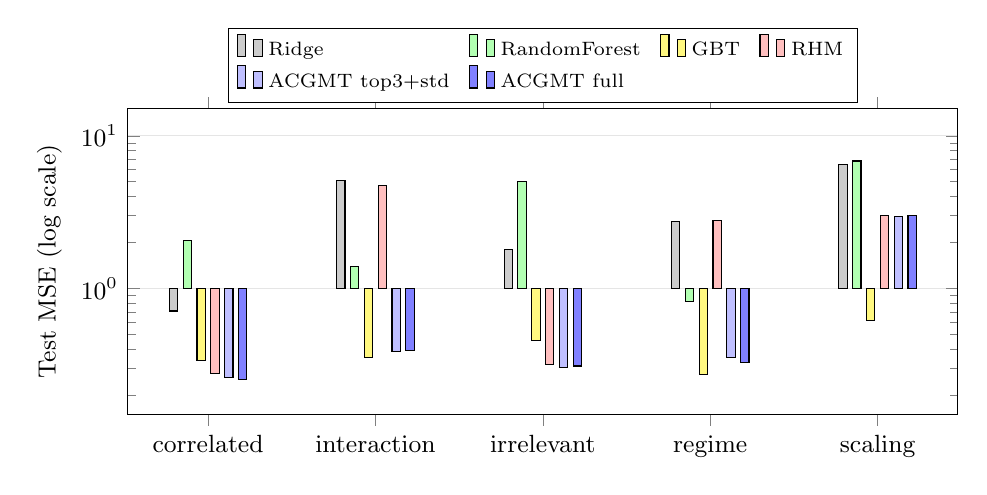
\begin{tikzpicture}
\begin{axis}[
    ybar,
    width=\textwidth,
    height=0.45\textwidth,
    ymode=log,
    ylabel={Test MSE (log scale)},
    symbolic x coords={correlated, interaction, irrelevant, regime, scaling},
    xtick=data,
    x tick label style={font=\small},
    tick label style={font=\small},
    label style={font=\small},
    ymin=0.15, ymax=15,
    bar width=3pt,
    enlarge x limits=0.12,
    legend style={at={(0.5,1.02)}, anchor=south, legend columns=4, font=\scriptsize,
                  /tikz/every even column/.append style={column sep=5pt}},
    legend cell align={left},
    grid=major,
    grid style={gray!20},
    ymajorgrids=true,
    xmajorgrids=false,
]
\addplot[fill=gray!40] coordinates {
    (correlated, 0.711) (interaction, 5.102) (irrelevant, 1.810)
    (regime, 2.758) (scaling, 6.492)};
\addplot[fill=green!30] coordinates {
    (correlated, 2.068) (interaction, 1.387) (irrelevant, 5.002)
    (regime, 0.820) (scaling, 6.833)};
\addplot[fill=yellow!50] coordinates {
    (correlated, 0.335) (interaction, 0.352) (irrelevant, 0.453)
    (regime, 0.274) (scaling, 0.615)};
\addplot[fill=red!25] coordinates {
    (correlated, 0.277) (interaction, 4.746) (irrelevant, 0.316)
    (regime, 2.791) (scaling, 3.020)};
\addplot[fill=blue!25] coordinates {
    (correlated, 0.259) (interaction, 0.385) (irrelevant, 0.303)
    (regime, 0.352) (scaling, 2.963)};
\addplot[fill=blue!50] coordinates {
    (correlated, 0.253) (interaction, 0.389) (irrelevant, 0.310)
    (regime, 0.325) (scaling, 2.998)};
\legend{Ridge, RandomForest, GBT, RHM, ACGMT top3+std, ACGMT full}
\end{axis}
\end{tikzpicture}
\caption{Test MSE comparison across datasets (log scale). RHM fails on the interaction and regime datasets (tall red bars), while ACGMT variants (blue) reduce error by an order of magnitude. GBT (yellow) is strongest on scaling and interaction. ACGMT beats GBT on correlated and irrelevant data.}\label{fig:comparison}
\end{figure}

\subsubsection{Ablation Study}

Table~\ref{tab:ablations} summarizes the ablations.

\begin{table}[ht]
\centering
\caption{Ablation study: test MSE across datasets.}\label{tab:ablations}
\resizebox{\textwidth}{!}{
\begin{tabular}{lcccccccccc}
\toprule
\textbf{Dataset} & \multicolumn{4}{c}{\textbf{Top-$k$}} & \multicolumn{2}{c}{\textbf{Standardize}} & \multicolumn{2}{c}{\textbf{Grid}} & \multicolumn{2}{c}{\textbf{Pruning}} \\
\cmidrule(lr){2-5}\cmidrule(lr){6-7}\cmidrule(lr){8-9}\cmidrule(lr){10-11}
 & top-1 & top-2 & top-3 & top-5 & no-std & with-std & adaptive & fixed & no-prune & with-prune \\
\midrule
correlated  & 0.265 & 0.259 & 0.259 & 0.259 & 0.259 & 0.259 & 0.259 & 0.259 & 0.263 & 0.253 \\
interaction & 0.528 & 0.385 & 0.385 & 0.385 & 0.385 & 0.385 & 0.374 & 0.385 & 0.388 & 0.389 \\
irrelevant  & 0.336 & 0.310 & 0.303 & 0.304 & 0.303 & 0.303 & 0.304 & 0.303 & 0.316 & 0.310 \\
regime      & 2.441 & 0.352 & 0.352 & 0.353 & 0.352 & 0.352 & 0.337 & 0.352 & 0.331 & 0.325 \\
scaling     & 5.122 & 3.869 & 2.963 & 1.719 & 1.719 & 2.963 & 3.080 & 2.963 & 3.002 & 2.998 \\
\bottomrule
\end{tabular}}
\end{table}

Figures~\ref{fig:topk} and~\ref{fig:ablation_panels} present the ablation results graphically. The ablations support four conclusions.

\paragraph{Top-$k$ screening is the dominant enhancement.}
Moving from top-1 to top-2 or top-3 produces the largest single gains. On the regime dataset, test MSE drops from 2.441 to 0.352; on the interaction dataset it drops from 0.528 to 0.385; on the scaling dataset it drops from 5.122 to 2.963 by top-3 and to 1.719 by top-5. The main weakness of RHM is therefore not merely threshold search, but the early commitment to a single splitting feature.

\paragraph{Standardization is not uniformly helpful.}
We expected node-wise standardization to stabilize coefficient ranking, but in these experiments it is neutral on four datasets and harmful on the scaling stress test. This is a useful negative result. Once top-$k$ screening is already exploring multiple features, naive standardization can alter the ranking in ways that do not improve split quality.

\paragraph{Adaptive threshold search helps when breakpoint precision matters.}
Adaptive refinement improves the regime dataset from 0.352 to 0.337 and the interaction dataset from 0.385 to 0.374, while remaining nearly neutral elsewhere. Its effect is therefore smaller than top-$k$ screening but still meaningful for problems with sharper local transitions.

\paragraph{Pruning is a small but generally positive refinement.}
In the clean pruning ablation, pruning improves correlated, irrelevant, regime, and scaling data, and is effectively neutral on interaction. The gains are modest, which is exactly what one would expect from a bottom-up regularization step rather than a fundamentally different split-selection mechanism.

\begin{figure}[ht]
\centering
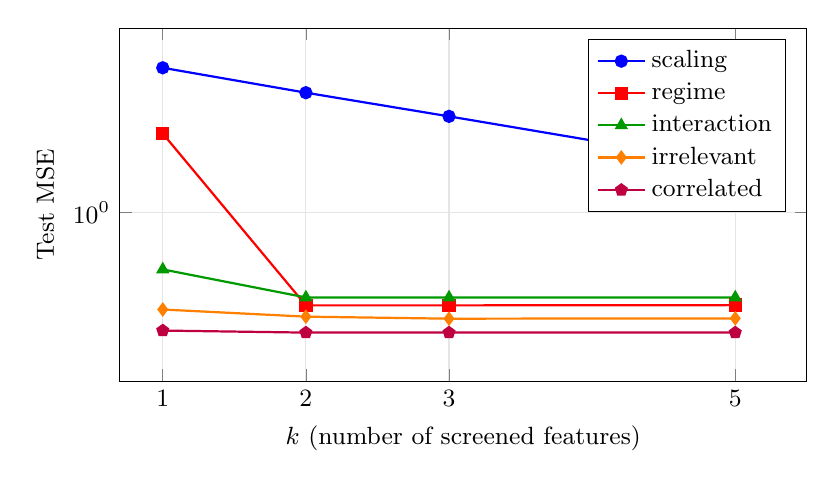
\begin{tikzpicture}
\begin{axis}[
    width=0.85\textwidth,
    height=0.5\textwidth,
    xlabel={$k$ (number of screened features)},
    ylabel={Test MSE},
    ymode=log,
    xmin=0.7, xmax=5.5,
    xtick={1,2,3,5},
    ymin=0.15, ymax=8,
    grid=major,
    grid style={gray!20},
    tick label style={font=\small},
    label style={font=\small},
    legend style={at={(0.97,0.97)}, anchor=north east, font=\small},
    legend cell align={left},
]
\addplot[thick, mark=*, blue] coordinates {(1,5.122) (2,3.869) (3,2.963) (5,1.719)};
\addlegendentry{scaling}
\addplot[thick, mark=square*, red] coordinates {(1,2.441) (2,0.352) (3,0.352) (5,0.353)};
\addlegendentry{regime}
\addplot[thick, mark=triangle*, green!60!black] coordinates {(1,0.528) (2,0.385) (3,0.385) (5,0.385)};
\addlegendentry{interaction}
\addplot[thick, mark=diamond*, orange] coordinates {(1,0.336) (2,0.310) (3,0.303) (5,0.304)};
\addlegendentry{irrelevant}
\addplot[thick, mark=pentagon*, purple] coordinates {(1,0.265) (2,0.259) (3,0.259) (5,0.259)};
\addlegendentry{correlated}
\end{axis}
\end{tikzpicture}
\caption{Effect of top-$k$ feature screening on test MSE (log scale). The largest gains occur from $k\!=\!1$ to $k\!=\!2$. The regime dataset drops from 2.44 to 0.35---a $7\times$ reduction---when the algorithm considers a second feature. Scaling continues to improve through $k\!=\!5$.}\label{fig:topk}
\end{figure}

\begin{figure}[ht]
\centering
\begin{minipage}[t]{0.48\textwidth}
\centering
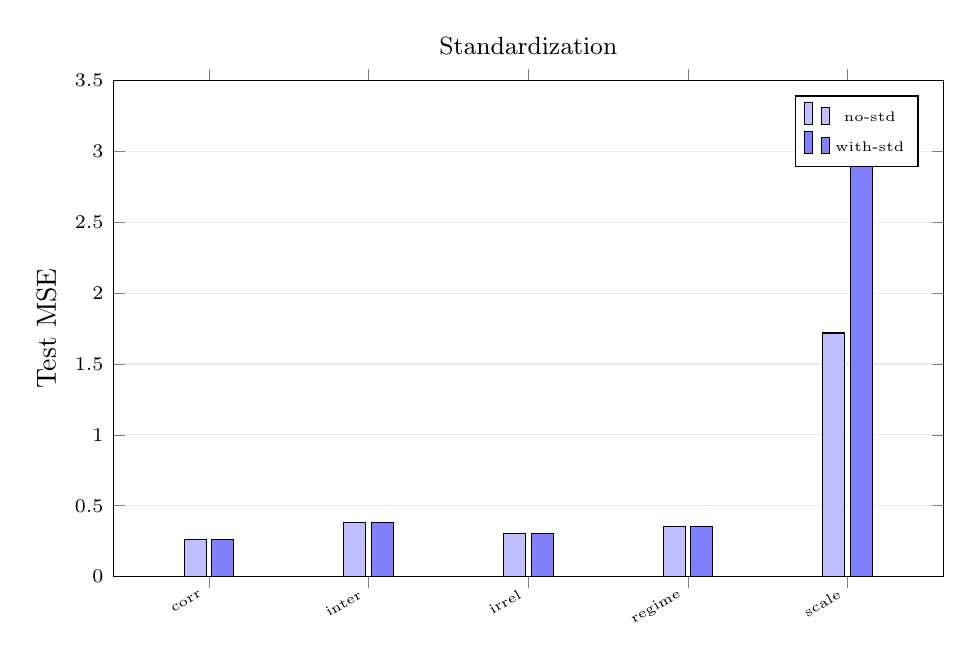
\begin{tikzpicture}
\begin{axis}[
    ybar,
    width=\textwidth, height=0.65\textwidth,
    title={\small Standardization},
    ylabel={Test MSE},
    symbolic x coords={corr, inter, irrel, regime, scale},
    xtick=data,
    x tick label style={font=\tiny, rotate=30, anchor=east},
    tick label style={font=\scriptsize},
    ymin=0, ymax=3.5,
    bar width=8pt,
    enlarge x limits=0.15,
    legend style={at={(0.97,0.97)}, anchor=north east, font=\tiny},
    grid=major, grid style={gray!15}, ymajorgrids=true, xmajorgrids=false,
]
\addplot[fill=blue!25] coordinates {(corr,0.259) (inter,0.385) (irrel,0.303) (regime,0.352) (scale,1.719)};
\addplot[fill=blue!50] coordinates {(corr,0.259) (inter,0.385) (irrel,0.303) (regime,0.352) (scale,2.963)};
\legend{no-std, with-std}
\end{axis}
\end{tikzpicture}
\end{minipage}\hfill
\begin{minipage}[t]{0.48\textwidth}
\centering
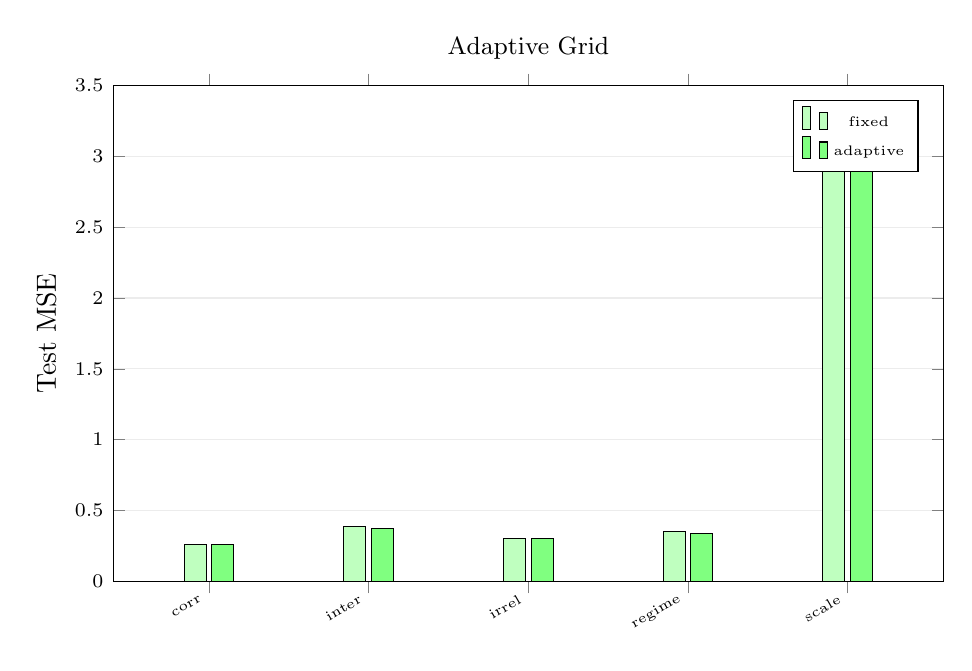
\begin{tikzpicture}
\begin{axis}[
    ybar,
    width=\textwidth, height=0.65\textwidth,
    title={\small Adaptive Grid},
    ylabel={Test MSE},
    symbolic x coords={corr, inter, irrel, regime, scale},
    xtick=data,
    x tick label style={font=\tiny, rotate=30, anchor=east},
    tick label style={font=\scriptsize},
    ymin=0, ymax=3.5,
    bar width=8pt,
    enlarge x limits=0.15,
    legend style={at={(0.97,0.97)}, anchor=north east, font=\tiny},
    grid=major, grid style={gray!15}, ymajorgrids=true, xmajorgrids=false,
]
\addplot[fill=green!25] coordinates {(corr,0.259) (inter,0.385) (irrel,0.303) (regime,0.352) (scale,2.963)};
\addplot[fill=green!50] coordinates {(corr,0.259) (inter,0.374) (irrel,0.304) (regime,0.337) (scale,3.080)};
\legend{fixed, adaptive}
\end{axis}
\end{tikzpicture}
\end{minipage}

\vspace{8pt}

\begin{minipage}[t]{0.48\textwidth}
\centering
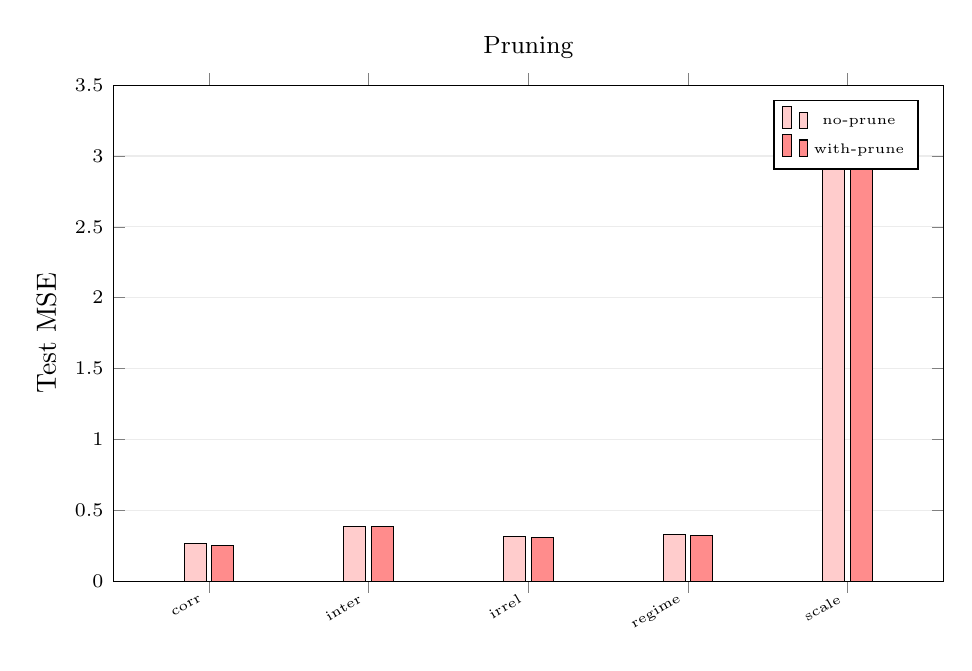
\begin{tikzpicture}
\begin{axis}[
    ybar,
    width=\textwidth, height=0.65\textwidth,
    title={\small Pruning},
    ylabel={Test MSE},
    symbolic x coords={corr, inter, irrel, regime, scale},
    xtick=data,
    x tick label style={font=\tiny, rotate=30, anchor=east},
    tick label style={font=\scriptsize},
    ymin=0, ymax=3.5,
    bar width=8pt,
    enlarge x limits=0.15,
    legend style={at={(0.97,0.97)}, anchor=north east, font=\tiny},
    grid=major, grid style={gray!15}, ymajorgrids=true, xmajorgrids=false,
]
\addplot[fill=red!20] coordinates {(corr,0.263) (inter,0.388) (irrel,0.316) (regime,0.331) (scale,3.002)};
\addplot[fill=red!45] coordinates {(corr,0.253) (inter,0.389) (irrel,0.310) (regime,0.325) (scale,2.998)};
\legend{no-prune, with-prune}
\end{axis}
\end{tikzpicture}
\end{minipage}\hfill
\begin{minipage}[t]{0.48\textwidth}
\centering
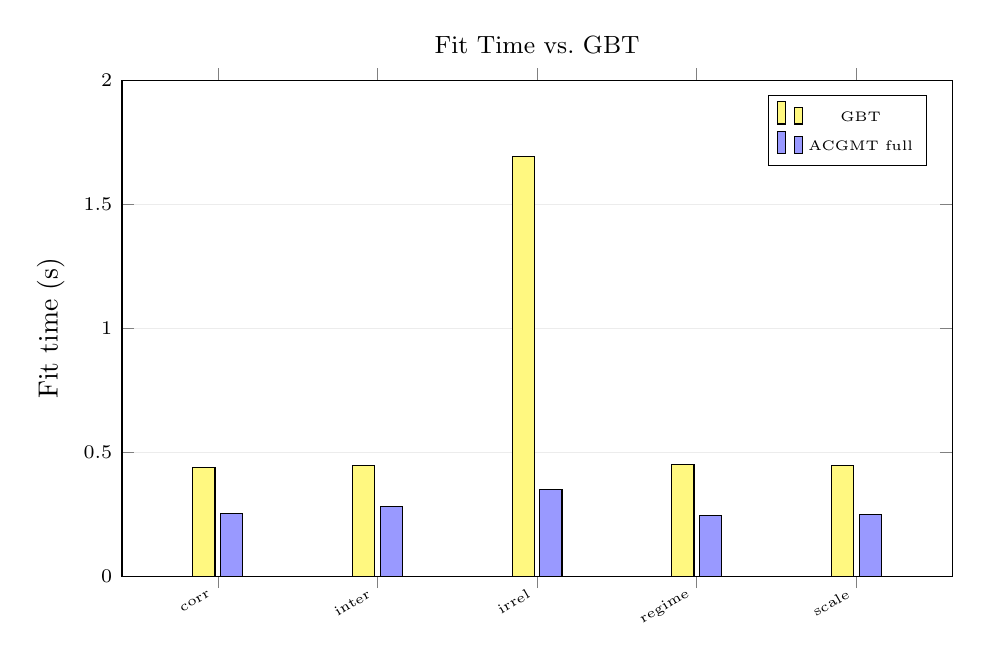
\begin{tikzpicture}
\begin{axis}[
    ybar,
    width=\textwidth, height=0.65\textwidth,
    title={\small Fit Time vs.\ GBT},
    ylabel={Fit time (s)},
    symbolic x coords={corr, inter, irrel, regime, scale},
    xtick=data,
    x tick label style={font=\tiny, rotate=30, anchor=east},
    tick label style={font=\scriptsize},
    ymin=0, ymax=2.0,
    bar width=8pt,
    enlarge x limits=0.15,
    legend style={at={(0.97,0.97)}, anchor=north east, font=\tiny},
    grid=major, grid style={gray!15}, ymajorgrids=true, xmajorgrids=false,
]
\addplot[fill=yellow!50] coordinates {(corr,0.438) (inter,0.446) (irrel,1.692) (regime,0.450) (scale,0.447)};
\addplot[fill=blue!40] coordinates {(corr,0.252) (inter,0.281) (irrel,0.349) (regime,0.244) (scale,0.251)};
\legend{GBT, ACGMT full}
\end{axis}
\end{tikzpicture}
\end{minipage}
\caption{Ablation panels. Top-left: standardization is neutral on 4/5 datasets and harmful on scaling. Top-right: adaptive grid refinement helps regime (0.352$\to$0.337) and interaction (0.385$\to$0.374). Bottom-left: pruning gives small improvements on 4/5 datasets. Bottom-right: ACGMT full fits faster than GBT on all datasets.}\label{fig:ablation_panels}
\end{figure}

\subsubsection{Complexity-Contextualized Comparison: Performance-Equivalent Boosting Budgets}

The main comparison in Table~\ref{tab:main} evaluates ACGMT against gradient boosting regression (GBR) with 100 depth-4 estimators. This is a useful practical comparison, but it is not complexity-matched: a single depth-4 model tree is evaluated against an additive ensemble of one hundred boosted trees, each fitted to residuals of the previous. To contextualize this gap, we conduct a complexity sweep over GBR ensemble sizes ($n_{\text{estimators}} \in \{1, 2, 4, 8, 16, 32, 64, 100\}$, all at depth 4) and identify, for each dataset, the smallest ensemble size at which GBR first matches or exceeds the test $R^2$ of ACGMT (depth~4, full configuration). We refer to this quantity as the \emph{empirical performance-equivalent boosting budget}. This analysis does not constitute a proof of equivalent model capacity---the representational structures of a single linear-model tree and a boosted ensemble remain fundamentally distinct---but it provides an empirically grounded basis for contextualizing the single-tree results within an ensemble complexity scale.

The results reveal a pronounced dependence on problem structure. On the two synthetic datasets designed to exhibit piecewise-linear or axis-aligned structure---the correlated-features and irrelevant-features benchmarks---a single ACGMT tree achieves $R^2$ of 0.983 and 0.992 respectively, and GBR does not match either value within the tested sweep of 100 estimators (GBR at 100 estimators reaches 0.978 and 0.988). These results indicate that the inductive bias of ACGMT, which partitions the input space into locally linear regions guided by regression coefficient structure, is particularly well-suited to problems where the generative process is itself approximately piecewise linear.

On three moderately nonlinear benchmarks---the interaction, regime, and friedman1 datasets---ACGMT achieves $R^2$ values of 0.953, 0.914, and 0.850 respectively. GBR requires approximately 32 estimators to match performance on the regime and friedman1 datasets, and between 32 and 64 estimators on the interaction dataset. That GBR at 100 estimators ultimately reaches higher values (0.957, 0.928, and 0.937) confirms that boosting retains a peak-accuracy advantage on these problems, but the performance-equivalent boosting budget of roughly 32 estimators indicates that ACGMT's single-tree solution is competitive with a meaningfully sized ensemble.

On california housing, concrete compressive strength, and airfoil self-noise, GBR reaches ACGMT-level performance at approximately 16 estimators, and larger ensembles ultimately achieve higher peak accuracy ($R^2$ of 0.811, 0.923, and 0.884 against ACGMT's 0.696, 0.838, and 0.702). Diabetes behaves differently: ACGMT (0.383) remains slightly above GBR(100) (0.352), while pruning collapses the tree to depth~1 across all tested depths, suggesting limited recoverable piecewise-linear structure under the current configuration.

The two remaining datasets represent the clearest limits of the ACGMT approach. On the yacht hydrodynamics dataset, ACGMT achieves an $R^2$ of only 0.577, and GBR at 4~estimators already approaches this value (approximately 0.55), with GBR at 100~estimators reaching 0.998. Pruning again collapses ACGMT to a depth-1 tree, consistent with a strongly nonlinear response surface that piecewise-linear partitioning cannot efficiently represent. On the scaling benchmark, ACGMT reaches 0.854 (improving through depth~5 to 0.868), while GBR requires approximately 32 estimators to match and ultimately achieves 0.970 at 100 estimators. On such problems, boosting with many estimators provides substantially higher peak accuracy, and ACGMT should not be expected to close that gap.

The complexity sweep also reveals a structural advantage in prediction cost. At inference time, ACGMT traverses a single tree and evaluates one local linear model (a dot product of $d$ coefficients), whereas GBR must traverse and sum the outputs of all $n_{\text{estimators}}$ trees. Table~\ref{tab:predict_time} reports mean prediction time over five seeds. On california housing ($m = 4{,}128$ test samples), ACGMT (depth~4) predicts in 0.39\,ms compared to 4.45\,ms for GBR(100)---an $11\times$ speedup. On friedman1 ($m = 1{,}000$), the ratio is $8\times$ (0.18\,ms vs 1.46\,ms). Even at the performance-equivalent ensemble size of GBR(32), ACGMT (depth~4) predicts $2$--$4\times$ faster. This advantage is a direct consequence of the single-tree architecture: prediction cost scales with tree depth rather than ensemble size, making ACGMT particularly attractive in deployment settings where prediction latency is constrained.

\begin{table}[ht]
\centering
\caption{Mean prediction time (ms) over 5 seeds. ACGMT predicts faster than GBR at all ensemble sizes because it traverses a single tree and evaluates one linear model per sample.}\label{tab:predict_time}
\begin{tabular}{lccccc}
\toprule
\textbf{Dataset} & \textbf{$m$} & \textbf{ACGMT (d=4)} & \textbf{GBR(32)} & \textbf{GBR(100)} & \textbf{Speedup} \\
\midrule
california  & 4,128 & 0.39 & 1.75 & 4.45 & $11\times$ \\
friedman1   & 1,000 & 0.18 & 0.50 & 1.46 & $8\times$ \\
interaction & 1,000 & 0.32 & 0.39 & 1.17 & $4\times$ \\
concrete    & 206   & 0.07 & 0.10 & 0.38 & $5\times$ \\
airfoil     & 301   & 0.14 & 0.12 & 0.59 & $4\times$ \\
\bottomrule
\end{tabular}
\end{table}

Taken together, these results provide a more contextualized comparison between ACGMT and gradient boosting. ACGMT is not uniformly competitive with GBR across all problem classes, nor should it be interpreted as a drop-in replacement for high-capacity ensembles. However, on datasets with structured or approximately piecewise-linear relationships, a single ACGMT tree attains the test performance that GBR reaches only after a nontrivial number of boosting stages---while predicting several times faster. This suggests that, in such regimes, ACGMT can offer a favorable tradeoff between predictive performance, prediction latency, and model inspectability.

%% TODO: Add complexity-curve figure
%% Figure: test R^2 vs GBR ensemble size, with ACGMT horizontal reference line

\section{Discussion}\label{sec:discussion}

\subsection{RHM: Advantages and Limitations}

The RHM experiments confirm that coefficient-guided model trees can outperform a global Ridge baseline on non-linear data with quadratic and interaction structure. The key advantages of the RHM design are threefold.

\paragraph{Linear interpretability within regions.} Unlike CART leaves (scalar constants), RHM leaves provide a full linear equation, enabling covariate-level attribution within each region.

\paragraph{Efficiency of coefficient-guided splitting.} By using Ridge coefficients to select the splitting feature, RHM avoids the $O(d)$-factor cost of CART's exhaustive feature search while still using data-driven evidence for the choice.

\paragraph{Regularised leaf models.} Ridge regression at the leaves prevents overfitting of individual leaf models, particularly important when deep trees produce small partitions.

The limitations of RHM are equally clear. The feature with the largest Ridge coefficient in the current partition is not guaranteed to be the optimal splitting feature according to the MSE criterion. The fixed percentile grid of 9 candidate split points may miss optimal thresholds that lie between percentiles. Hard binary routing creates discontinuities at region boundaries. And the algorithm does not include post-hoc pruning or cross-validation for depth selection, requiring external depth tuning.

These limitations motivate the progression from RHM to ACGMT described in Section~\ref{sec:acgmt}.

\subsection{ACGMT: What the Experiments Imply}

The ACGMT experiments suggest that coefficient-guided model trees are viable, but only when the coefficient signal is used as a \emph{screening tool} rather than a hard one-feature decision rule. This is the central lesson of the ACGMT study. RHM's top-1 heuristic fails badly on interaction and regime data; once the search is expanded to a small set of plausible features, the method becomes far more robust.

The results also clarify what ACGMT is \emph{not}. It is not a universal replacement for strong tree ensembles. Gradient boosting remains superior on strongly nonlinear problems (yacht, scaling) and achieves higher peak accuracy on most real-world datasets when given a large ensemble budget. Nor does every proposed enhancement help equally: top-$k$ screening is the clear driver of improvement, adaptive threshold refinement provides targeted gains, pruning gives small regularization benefits, and standardization is at best mixed.

The complexity sweep against gradient boosting (Section~\ref{sec:experiments}) adds an important nuance. The analysis does not imply that ACGMT and GBR possess equivalent representational capacity; rather, it establishes empirically that on several structured regression problems, the effective accuracy obtained from a single interpretable model tree falls within the range that GBR spans during its early-to-middle boosting iterations, before further estimators yield diminishing returns. On problems with approximately piecewise-linear structure, ACGMT matches the performance that GBR requires roughly 32 or more estimators to attain. On strongly nonlinear targets, GBR overtakes ACGMT with as few as 4--16 estimators. This pattern is consistent with the view that coefficient-guided model trees are most valuable when the underlying relationship is structured enough to be well-approximated by a small number of local linear models.

These observations lead to a more precise methodological claim. The value of coefficient-guided model trees lies not in a single heuristic, but in a family of constrained search strategies that trade exhaustive split search for a guided restricted search. ACGMT represents one such strategy, and the hierarchy of importance established by ablation---top-$k$ first, adaptive grid and pruning conditional, standardization cautious---is itself a key finding.

There are clear limitations to the present study. First, the comparison does not include an external exhaustive model-tree implementation (e.g., M5'); the focus is on the progression from RHM to ACGMT and on standard tabular baselines. Second, the present RHM implementation uses row-wise prediction, making fit time the cleaner efficiency metric compared to ACGMT's vectorized inference. Third, on datasets with very few samples (diabetes, yacht), pruning collapses the tree to depth~1, preventing meaningful evaluation of the tree-building enhancements.

\subsection{Future Directions}

\begin{enumerate}
    \item[(a)] Replacing the coefficient-based heuristic with a fast approximate feature search (e.g., random subset of features) or hybrid strategy for better split quality at moderate cost.
    \item[(b)] Implementing M5'-style smoothing across leaf boundaries to improve continuity of the piecewise linear predictor.
    \item[(c)] Extending to multi-output regression by replacing Ridge with multi-output Ridge at each node and leaf.
    \item[(d)] Integrating cross-validated depth selection or cost-complexity pruning into the RHM/ACGMT framework.
    \item[(e)] Investigating the theoretical regime in which top-$k$ screening achieves the same convergence guarantees as exhaustive feature search.
    \item[(f)] Comparing against external model-tree implementations (e.g., M5', PILOT, PINE) on standardized benchmark suites.
\end{enumerate}

\section{Conclusion}\label{sec:conclusion}

This paper presented a unified development of coefficient-guided model trees for piecewise linear regression, tracing the progression from a minimal baseline to a robust adaptive variant.

The Recursive Hybrid Model (RHM) established that a Ridge-coefficient-guided feature selection heuristic---selecting the splitting axis as the feature with the largest absolute coefficient magnitude---produces a clean, analysable algorithm with training complexity $O(D \cdot n \cdot d^2)$, inference complexity $O(m(D+d))$, and the classical $O(h^2)$ piecewise linear convergence rate in idealised settings. Empirical evaluation confirmed that RHM consistently outperforms a global Ridge baseline on synthetic non-linear data, with gains increasing with depth before diminishing returns set in.

The preceding analysis also identified the primary weakness of the top-1 heuristic: early commitment to a single splitting feature causes failures on data with scaling distortions, correlated predictors, and regime-dependent structure. The Adaptive Coefficient-Guided Model Tree (ACGMT) addressed this by promoting the coefficient signal from a hard decision rule to a screening device: the algorithm ranks features by coefficient magnitude, retains the top-$k$ candidates, and evaluates each for the best split. Ablation experiments on five synthetic stress tests showed that this single change is the dominant improvement---test MSE dropped by an order of magnitude on interaction and regime datasets when moving from top-1 to top-2 or top-3. Adaptive threshold refinement and validation-aware pruning provided supplementary, context-dependent gains; standardization was neutral to harmful.

A complexity sweep over gradient boosting ensemble sizes provides further context. On datasets with approximately piecewise-linear generative structure, a single ACGMT tree attains the predictive performance that gradient boosting reaches only after accumulating roughly 32 or more estimators, while remaining a fully inspectable model whose local linear components can be directly examined. On strongly nonlinear problems, boosting with many estimators achieves substantially higher peak accuracy, and practitioners should regard these cases as outside the method's primary domain of applicability.

The broader implication is that coefficient-guided model trees should be understood as \emph{adaptive search procedures}, not one-shot heuristics. The resulting ACGMT remains a single interpretable tree and significantly improves over the original coefficient-guided baseline on the problem classes where the baseline fails. The choice between ACGMT and a boosted ensemble should be guided by the degree to which interpretability and local linearity are operationally valued: on structured problems where the two approaches reach comparable accuracy, ACGMT provides fully inspectable local linear models at the cost of reduced peak performance on targets that exhibit complex global nonlinearity.

\bibliographystyle{plainnat}

\begin{thebibliography}{12}

\bibitem[Breiman et~al.(1984)]{breiman1984}
Breiman, L., Friedman, J., Olshen, R., \& Stone, C. (1984).
\newblock \emph{Classification and Regression Trees}.
\newblock Wadsworth.

\bibitem[Breiman(2001)]{breiman2001rf}
Breiman, L. (2001).
\newblock Random Forests.
\newblock \emph{Machine Learning}, 45(1), 5--32.

\bibitem[Cerlymarco(2021)]{cerlymarco2021}
Cerlymarco. (2021).
\newblock linear-tree: A python library to build Model Trees with Linear Models at the leaves.
\newblock GitHub. \url{https://github.com/cerlymarco/linear-tree}

\bibitem[Friedman(1979)]{friedman1979}
Friedman, J.~H. (1979).
\newblock A Tree-Structured Approach to Nonparametric Multiple Regression.
\newblock In T.~Gasser \& M.~Rosenblatt (Eds.), \emph{Smoothing Techniques for Curve Estimation}, Lecture Notes in Mathematics, vol.~757. Springer.

\bibitem[Friedman(1991)]{friedman1991}
Friedman, J.~H. (1991).
\newblock Multivariate Adaptive Regression Splines.
\newblock \emph{The Annals of Statistics}, 19(1), 1--67.

\bibitem[Friedman(2001)]{friedman2001gbm}
Friedman, J.~H. (2001).
\newblock Greedy Function Approximation: A Gradient Boosting Machine.
\newblock \emph{The Annals of Statistics}, 29(5), 1189--1232.

\bibitem[Hansen(2000)]{hansen2000}
Hansen, B.~E. (2000).
\newblock Sample Splitting and Threshold Estimation.
\newblock \emph{Econometrica}, 68(3), 575--603.

\bibitem[Hoerl \& Kennard(1970)]{hoerl1970}
Hoerl, A.~E., \& Kennard, R.~W. (1970).
\newblock Ridge Regression: Biased Estimation for Nonorthogonal Problems.
\newblock \emph{Technometrics}, 12(1), 55--67.

\bibitem[Li et~al.(2024)]{li2024}
Li, Z., et~al. (2024).
\newblock PINE: Efficient yet Effective Piecewise Linear Trees.
\newblock \emph{SC24 Supercomputing Conference Proceedings}.
\newblock \url{https://sc24.supercomputing.org/proceedings/poster/poster_files/post258s2-file3.pdf}

\bibitem[Quinlan(1992)]{quinlan1992}
Quinlan, J.~R. (1992).
\newblock Learning with Continuous Classes.
\newblock \emph{Proceedings of the 5th Australian Joint Conference on Artificial Intelligence}, pp.~343--348.

\bibitem[Raymaekers et~al.(2024)]{raymaekers2024}
Raymaekers, J., Rousseeuw, P.~J., Verdonck, T., \& Yao, R. (2024).
\newblock Fast Linear Model Trees by PILOT.
\newblock \emph{Machine Learning}.
\newblock \url{https://doi.org/10.1007/s10994-024-06590-3}

\bibitem[Wang \& Witten(1997)]{wang1997}
Wang, Y., \& Witten, I.~H. (1997).
\newblock Induction of Model Trees for Predicting Continuous Classes.
\newblock \emph{Proceedings of the European Conference on Machine Learning}, pp.~128--137.

\end{thebibliography}

\end{document}
